% This document provides the style to be used for a MSc Thesis at the
% Parallel and Distributed Systems group
\documentclass[11pt,twoside,a4paper,openright]{report}

% math packages
\usepackage{amsmath}
\usepackage{amssymb}

% textblocks for title page
\usepackage[absolute]{textpos}

% use babel for proper hyphenation
\usepackage[british]{babel}

% Graphics: different for pdflatex or dvi output, choose one
%%\usepackage[dvips]{graphicx}
%%\usepackage[pdftex]{graphicx}
\usepackage{graphicx}

\usepackage{epstopdf}
\usepackage{rotating}
\usepackage{subfigure}
\usepackage[table,xcdraw]{xcolor}

\usepackage{forest}
\usepackage{caption}
\usepackage{enumitem}
\usepackage{multirow}


\definecolor{folderbg}{RGB}{124,166,198}
\definecolor{folderborder}{RGB}{110,144,169}

\def\Size{4pt}
\tikzset{
	folder/.pic={
		\filldraw[draw=folderborder,top color=folderbg!50,bottom color=folderbg]
		(-1.05*\Size,0.2\Size+5pt) rectangle ++(.75*\Size,-0.2\Size-5pt);  
		\filldraw[draw=folderborder,top color=folderbg!50,bottom color=folderbg]
		(-1.15*\Size,-\Size) rectangle (1.15*\Size,\Size);
	}
}

% FONT
\usepackage[scaled=.92]{helvet}
%\usepackage{times}

% for url's use "\url{http://www.google.com/}"
\usepackage{url}
\usepackage[plainpages=false]{hyperref} 

% Information that will be filled in at various points in the report
\newcommand{\reportTitle}{Sensing human activity with dark light}
\newcommand{\reportAuthor}{Hajo Kleingeld}
\newcommand{\reportEmail}{hajokleingeld@gmail.com}
\newcommand{\reportUrlEmail}{\href{mailto:\reportEmail}{\reportEmail}}
\newcommand{\reportMSC}{Embedded Systems} %{Embedded Systems}{Computer Engineering}{Computer Science}{Electrical Engineering}
\newcommand{\reportDate}{\today} %TODO: Dit is de datum van uitgifte van final versie aan de afstudeer commissie 
\newcommand{\presentationDate}{\today} %TODO: Dit is de datum van de afstudeerpresentatie 
\newcommand{\graduationCommittee}{
Prof. dr. K.G. Langendoen (Chair) & Delft University of Technology \\
dr. M. Zuniga (Daily Supervisor) & Delft University of Technology \\
dr. C. Doerr & Delft University of Technology \\
} % The order of listing the names: Graduation prof, supervisor(s), others ordered by title + alphabetical 
%examples: 
%prof. dr. ir. H. J. Sips (chair) & Delft University of Technology \\ 
%ir. dr. D. H. J. Epema           & Delft University of Technology \\ 
\newcommand{\reportAbstract}{TODO ABSTRACT}
\newcommand{\reportKeywords}{TODO KEYWORDS}

% For pdflatex
\pdfinfo{
   /Author (\reportAuthor)
   /Title  (\reportTitle)
   /Keywords (\reportKeywords)
}

\begin{document}

\pagenumbering{alph}
\pagestyle{empty}


% FRONTCOVER
%%\usepackage[total={210mm,297mm},left=0pt,bottom=0pt,top=0cm,right=0pt,headsep=0pt,head=0pt,showframe]{geometry}

%%\input{preambleL31958}
%%\begin{titlepage}
\begin {textblock*}{210mm}(0mm,0mm)
\noindent

\includegraphics[height=3.2cm]{pics/block}
\sffamily
\vspace{.8cm}
\begin{center}
\Large
Delft University of Technology\\
Master's Thesis in \reportMSC\\
\vspace{2cm}
\parbox{170mm}{\bfseries\centering\Huge\reportTitle}\\
\vspace{1cm}
\parbox{170mm}{\bfseries\centering\reportAuthor}

\end{center}
\end{textblock*}

\begin {textblock*}{210mm}[0.0,1.0](0mm,297mm)
\noindent
\hspace{1.89cm}


\hfill\parbox{5cm}{

\includegraphics[width=5cm]{pics/es_logo_cyan_black_rgb}}
\hspace*{2cm}\\

\vspace*{1.5cm}
\noindent

\includegraphics[width=\textwidth]{pics/TU_border_A4_L_front}
\end{textblock*}

\null\newpage


%%%%%%%%%%%%%%%%%%%%%%%%%%%%%%%%%%%%%%%%%%%%%%%%%%%%%%%%%%%%%%%%%%%%%%%%%%%%%%%
\hoffset=1.63cm
\oddsidemargin=0in
\evensidemargin=0in
\textwidth=5in

%%%%%%%%%%%%%%%%%%%%%%%%%%%%%%%%%%%%%%%%%%%%%%%%%%%%%%%%%%%%%%%%%%%%%%%%%%%%%%%
\parindent=1em

% EMPTY PAGE
\cleardoublepage

\pagestyle{plain}
\pagenumbering{roman}
\setcounter{page}{1}

% TITLE PAGE: page i (hidden)
\begin{titlepage}

  \begin{center}
  \null\vfill
    \begin{center}
    \LARGE{\reportTitle}
    \end{center}

    \vspace{3cm}

    \begin{large}
    Master's Thesis in \reportMSC
    \end{large}

    \vspace{1.5cm}

    \begin{normalsize}
    Embedded Software Section\\
    Faculty of Electrical Engineering, Mathematics and Computer Science\\
    Delft University of Technology\\
    Mekelweg 4, 2628 CD Delft, The Netherlands
    \end{normalsize}

    \vspace{2.0cm}

    \begin{normalsize}
    \reportAuthor \\
    \reportUrlEmail
    \end{normalsize}

    \vspace{1.0cm}

    % <MM> DD, YYYY
    \reportDate             %TODO: Dit is de datum van uitgifte van final versie aan de afstudeer commissie

  \vfill
  \end{center}

\end{titlepage}


% GRADUATION DATA AND ABSTRACT: pages ii and iii (hidden)
%De aankondiging bevat de spreker, titel, plaats, datum en tijd, samenstelling van de afstudeercommissie en een korte samenvatting (maximaal 25 regels).
\thispagestyle{empty}

\noindent \textbf{Author}\\
\begin{tabular}{l}
\reportAuthor{} (\reportUrlEmail)\\
\end{tabular}\\
\noindent \textbf{Title}\\
\begin{tabular}{l}
\reportTitle\\
\end{tabular}\\
\noindent \textbf{MSc presentation}\\
\begin{tabular}{l}
% <MM> DD, YYYY (like \today)
\presentationDate\\
\end{tabular}

\vspace{1.1cm}

\noindent \textbf{Graduation Committee}\\
\begin{tabular}{ll}
\graduationCommittee
\end{tabular}


\begin{abstract}
%What is the problem + why is it important
Nowadays, 19\% of the global energy consumption is used for lighting. For this reason, saving energy in lighting is vital. A simple way to save energy is to “simply” turn the lights off, or reduce the amount of light used when nobody is around. This thesis proposes a new method for luminaires to detect the presence of humans and objects which only uses a photodiode and a fraction of the light a luminaire normally emits, namely \textit{Dark Sensing}.

%What is my solution
Dark sensing works by sending out short flashes of light. These short flashes use little energy and are barely visible to the user. These flashes get reflected by the environment and received by a photodiode placed next to the light. By extracting a key feature of the received flash, we obtain a metric representing the surrounding area. If an object enters the observed area, the reflections of light will change. These changes will be noticed by the system, which triggers a detection resulting in the light being turned on.

%What follows from my solution
A prototype was created which shows the potential of the newly developed method. The prototype was tested in two different environments and detects between 73\% and 90\% of bypassing pedestrians, depending on the accepted false positive ratio (0 to 0.05).

\setcounter{page}{3}
\reportAbstract{}
\end{abstract}

\clearpage

%\setcounter{page}{4}

% EMPTY PAGE: page iv
\cleardoublepage

% OPTIONAL QUOTATION: page v
%\pagestyle{empty}

\null\vfill

\begin{center}
\emph{``TODO QUOTE''} -- TODO QUOTED PERSON
\end{center}

\vspace{10cm}

\clearpage


% EMPTY PAGE: page vi
%\cleardoublepage

% PREFACE: page v
\chapter*{Preface}
\addcontentsline{toc}{chapter}{Preface}
TODO MOTIVATION FOR RESEARCH TOPIC

\vspace{1\baselineskip}

\noindent
TODO ACKNOWLEDGEMENTS

\vspace{1\baselineskip}

\noindent
Hajo Kleingeld

\vspace{1\baselineskip}

\noindent
Delft, The Netherlands

\noindent
\today

% EMPTY PAGE: page vi
\cleardoublepage

% TABLE OF CONTENTS: starting at page vii
\tableofcontents

\cleardoublepage

\pagenumbering{arabic}
\setcounter{page}{1}

% INTRODUCTION: page 1
\chapter{Introduction}
\label{chp:introduction}
Nowadays, 19\% of the global energy consumption is used for lighting. For this reason, saving energy in lighting is vital. A simple way to save energy is to “simply” turn the lights off, or reduce the amount of light used when nobody is around. This thesis proposes a new method for luminaires to detect the presence of humans and objects, namely \textit{Dark Sensing}.

The idea of human sensing is not new. Everybody in the western world has walked into a room where the lights suddenly turned on once they entered. The most common method to create this effect is to make use of a PIR (passive-infrared) sensor. By monitoring the infra-red radiation (heat) in the area, it can detect changes in the environment and toggle the light based on these changes. This method works very well but has several drawbacks. The first is that it's unable to detect objects with the same surface temperature as the environment, for example a car where the engine has just been turned on. Another drawback is that the PIR method has no potential for communication without the addition of extra components. Dark sensing attempts to overcome these drawbacks by only using a photodiode and the light in the visible spectrum a luminaire normally emits.

This thesis explores the idea of detecting changes in the environment with reflections of visible light. The proposed system works in the following manner: If nothing is in the area, the light will be turned on, but outputting a very low light level. Some of the light will reflect off the environment back to the light source. This can be measured with the photodiode. The signal received is a measure of the illuminated area. If something were to change in that area, a car drives by for example, then the reflections in the environment will change and therefore the light perceived by the photodiode will change as well. These changes will then result in a detection by the system which will turn the light on at full brightness. An overview of the scenario can be seen in \ref{fig:Introduction}.

This method by itself does not save energy as the light used in the system is always turned on. If we are able to reduce the light output while maintaining the ability to pick up meaningful reflections, then the system would save energy. This can be achieved by turning the light on and off very quickly. Then, if the reflections are only measured when the light is fully turned on, we can capture a reflection while saving energy, because the light is only on part of the time.
\begin{figure}[]
	\centering     %%% not \center
	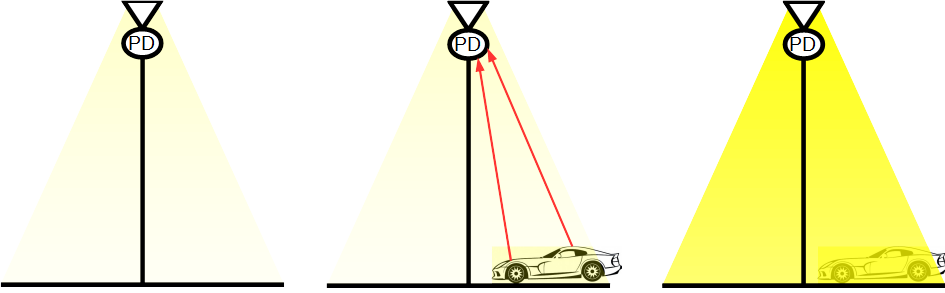
\includegraphics[width=120mm]{pics/SystemScenario.png}
	\caption{When no object is in the area, the luminaire will barely generate any light. If an object drives into the area, the reflections will be picked up by the photodiode, which will then turn the light on. \label{fig:Introduction}}
\end{figure}

The ultimate goal of the proposed system is to reduce the time the light needs to be on the nearly zero. This will lead to a light which barely consumes any energy while nobody is around but is still able to detect people, cars or other objects passing by. It might even be possible to decrease the light output to an amount which is invisible to the human eye, resulting in an unnoticeable, activity detecting, energy-saving device.

\section{Problem statement}
\label{Problem statement}
\textbf{Is it possible to create a system which can detect the activity of humans or objects by measuring reflections of visible light while being invisible to the human eye?}
\\
\\
This problem can be divided into three sub-questions:
\begin{itemize}\itemsep2pt
	\item How strong is a reflection obtained from a flash in a realistic scenario and how much does this reflection vary if an object enters the area?
	\item What are the challenges in obtaining reflections when the light is turned on for a very short time and how can they be tackled?
	\item What additional signals are received by the system (besides the reflection of the flash) and what algorithm can be used to convert the received signal in a reliable logical signal: Detection or no detection?
\end{itemize}

\section{Contributions}
\label{sec:Contributions}
This thesis proposes \textbf{Dark Sensing}, a system that uses reflections of a LED controlled with a low duty cycle (4\%), and therefore nearly invisible to the human eye, to detect changes in the surrounding area.
\begin{itemize}\itemsep2pt
	\item A model, estimating the change in signal (reflected light) when a object moves under, leaves or passes by the LED in different environments.
	\item A method to convert a captured reflection of the LED into a usable measure of the environment.
	\item An algorithm which analyses features of consecutive flashes and is capable of detecting objects moving under, leaving or passing through the illuminated area.
	\item A prototype capable of detecting 87\% of all humans passing by in a realistic environment.
\end{itemize}

\section{Organisation}
This thesis describes the development path of the new technique "Dark Sensing" from idea to a working prototype. Chapter 2 will present the required background knowledge to understand several choices made in this thesis and present the related work. In chapter 3 a model will be presented, which calculates the theoretical response of bypassing objects. Chapter 4 describes the created experimentation platform. Chapter 5 will focus on finding the ideal settings for generating an analysable flash and will explain what the best method is for extracting data from this flash. Chapter 6 explores the possibilities for analysing sets of consecutive flashes and proposes an algorithm to detect significant changes in the signal. Chapter 7 tests the prototype created and evaluates the performance of system. The thesis concludes with an evaluation of the new "Dark Sensing" technology and suggests several possible directions for future work.

% CHAPTERS ... For instance: History/Prior Work, Design/Implementation, Experiments
\chapter{Background and related work}

\section{Background}
\label{sec:Background}
This section presents the required field knowledge to understand this thesis. It therefore starts with an explanation on how a light source behaves when it turns on and off rapidly and why this is preferable over other light saving strategies. It then follows up with an explanation of how produced light travels and reflects off of surfaces.

\subsection{Dimming of an LED}
In this thesis, an LED will be used to illuminate the environment which will cause reflections in the room. It's therefore important to understand how the light responds to different methods of adjusting the light output, as this directly influences power of the reflections.

In general, there are two methods of dimming (reducing the light output of) an LED: Analogue and digital. A light which is dimmed in an analogue manner has its total light output reduced by reducing the current flowing into the LED. This leads to a light which has a constant light output directly proportional to the current flowing into the LED. If we for example want a light to produce 25\% of its normal light output, we simply supply it with a quarter of the current. A graphical representation of analogue dimming is shown in Figure \ref{fig:PWM} and is marked as "average power".

Digital dimming works in another way. Instead of controlling the amount of current flowing into the LED, we control the amount of time current is allowed to flow into the LED. This can be achieved by turning the LED on and off rapidly. If we for example want to reduce the light output of an LED to 25\% with the help of digital dimming, then we would turn the light on at full strength for 25\% of the time, while turning it off for 75\%, with the help of a Pulse Width Modulated (PWM) signal. A graphical representation of digital dimming is shown in Figure \ref{fig:PWM}.

The resulting light produced by both types of dimming are indistinguishable for humans if the switching frequency is high enough. Both methods have the same apparent brightness and use the same amount of power. For photo diodes however, there is a clear difference. The analogue signal will show up as a constant, but weak signal. The digital signal shows up as a square wave with high peaks (when the light is on) and valleys (when the light is off). This becomes especially apparent if we want the system to work at only 1\% of it's original illumination level. The signal dimmed in an analogue manner will be nearly invisible as it is turned on constantly at 1\% of it's original power. This in contrast to the digital signal, which only shows up for 1\% of the time, but at maximum power, resulting in a shorter but much brighter peak. Because the 1\% time constrain is no problem for an electronic system, it was chosen to explore Dark Sensing with this dimming method.

%turning on and off pattern
There is however a limit to how much the energy consumption can be reduced with digital dimming, if we want to be able to observe the signal with a photo diode. When an LED is turned on, it does not produce light at maximum intensity instantly\cite{LED_on}. It first has a short "turn-on delay" where the light does not output any light, followed by a "rise time" where the light "slowly" powers up until it has reached it's desired intensity level. A graphical representation of this process can be seen in figure \ref{fig:LedResponse}. This limit on digital dimming forces a hard minimum to the amount of digital dimming the system can work with and therefore limits the amount of energy it can save.

\begin{figure}[]
	\subfigure[]{\label{fig:PWM}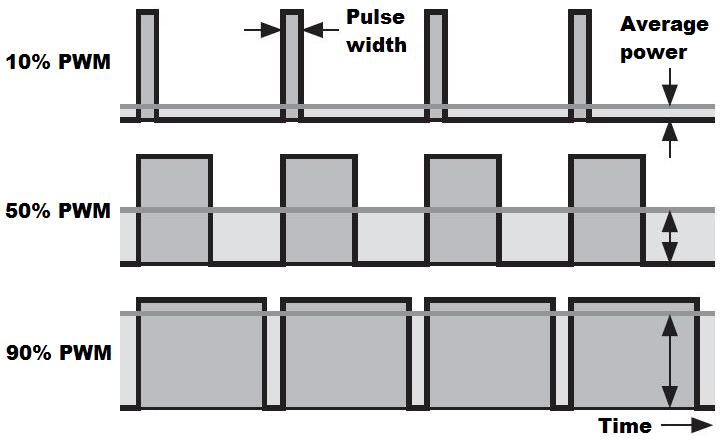
\includegraphics[width=60mm]{pics/PWM.png}}
	\subfigure[]{\label{fig:LedResponse}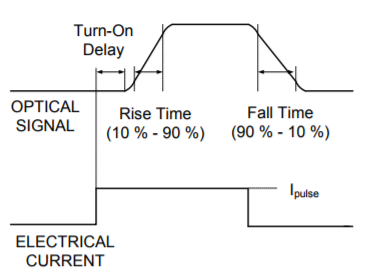
\includegraphics[width=60mm]{pics/LedResponse.png}}
	\caption{Figure (a) shows the difference between analogue and digital dimming, Figure (b) shows a realistic response of the light when a short electric pulse is applied\cite{LED_on}.\label{fig:LedOnTime}}
\end{figure}

\subsection{The Phong model}
\label{Model_explained}
When a light shines on a surface, some parts of the surface appear brighter than other parts. This is caused by three major factors:
\begin{itemize}[itemsep=-1ex,topsep=0pt]
	\item The light used to illuminate the wall and it's position relative to the wall.
	\item The surface of the wall itself.
	\item The position of the observer relative to the wall.
\end{itemize}
If all of these factors are known, then the complete pathing of the light can be approximated with the help of the Phong model. This section presents a simplified version of the Phong model which is used in chapter \ref{Model}. All used angles can be seen in Figure \ref{fig:model_overview}. The full model can be found in \cite{Advances_In_Optical_Communication}.

\begin{figure}
	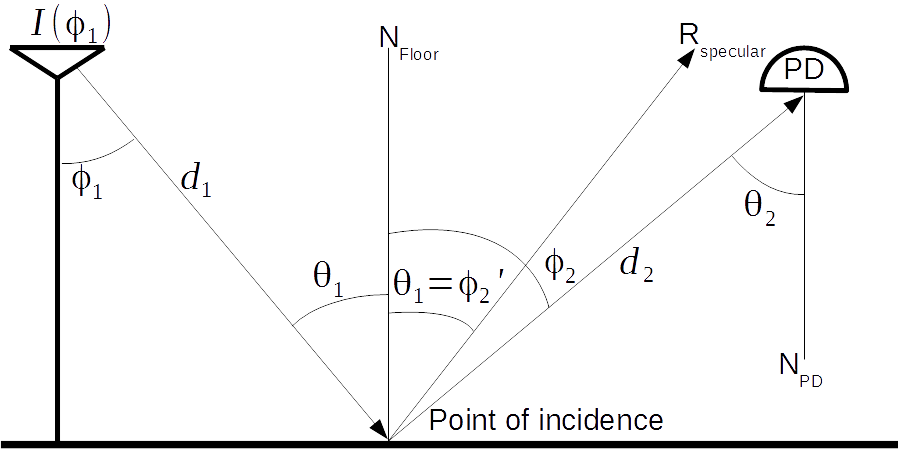
\includegraphics[width=\textwidth]{pics/single_light_post.png}
	\caption{Overview of angles, vectors and distances used in the model. It represents a street light illuminating the street (I). This light is then observed by a photo diode (PD), aimed at the ground. Note that $\phi$ always represents an exit angle and $\theta$ always represents an incidence angle.\label{fig:model_overview}}
\end{figure}

\subsubsection{Modelling an LED}
A light can be modelled if several parameters of the light are known, with the help of equation \ref{eq:I(phi)}. This formula describes how much light is leaving the light source at angle $\phi$ relative to the normal of the LED.
\begin{equation}
\label{eq:I(phi)}
I(\phi)=\Phi_{lum}\frac{\alpha+1}{2\pi}cos^\alpha(\phi_1)
\end{equation}
The equation consists of three parts. $\Phi_{lum}$ represents the total amount of light emitted in lumen by the LED. $cos^\alpha(\phi_1)$ represents the radiation pattern of the LED. $\alpha$ represents the order of Lambertian emission which describes the illumination pattern of the LED. If $\alpha$ is low (e.g. 1), then this equation represents a luminaire with a very wide spread of light, for example a street light. If $\alpha$ is high (e.g. 200+), then the light source is much more focused like a laser. An overview of $\alpha$ vales versus their angle is shown in Figure \ref{fig:cones_of_light}. $\frac{\alpha+1}{2\pi}$ is a normalisation factor that ensures that integrating equation \ref{eq:I(phi)} results in the total amount of light produced ($\Phi_{lum}$), as reshaping the cone of light with $\alpha$ would otherwise lead to a change in produced light. An example of a modelled light with $\alpha = 14.3$ and $\Phi_{lum} = 260lm$ can be seen in Figure \ref{fig:2lightcones}.

We can now take any light ray from the luminaire and calculate how much light hits a specific surface with the help of equation \ref{eq:E_hor}. This calculation also consists of three parts. The first part is the strength of the light ray calculated with equation \ref{eq:I(phi)}. The second part, $d$, represents the distance the light needs to travel before it hits the surface. The final variable, $\theta_1$, represents the incidence angle of the light ray on the surface.
\begin{equation}
\label{eq:E_hor}
E_{hor} = \frac{I(\phi_1)}{d^2} cos(\theta_1)
\end{equation}

%\begin{figure}
%	\centering     %%% not \center
%	\subfigure[]{\label{fig:Specs_a}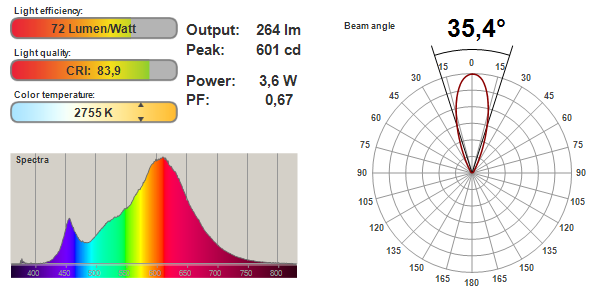
\includegraphics[width=68mm]{pics/LED_specs.png}}
%	\subfigure[Caclculated intensity pattern ]{\label{fig:Specs_b}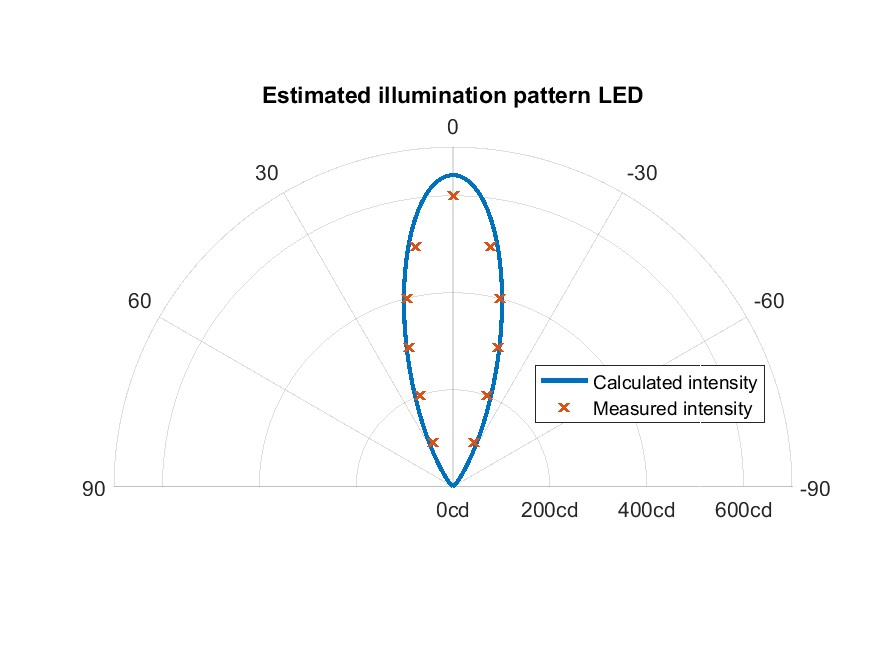
\includegraphics[width=52mm]{pics/polarplot_LED.png}}
%	\caption{Figure (a) shows measured specifications of an LED \cite{lamptest} where Figure (b) shows the estimated illumination pattern of the same LED with the described method.}
%\end{figure}

\begin{figure}
	\centering     %%% not \center
	\subfigure[]{\label{fig:cones_of_light}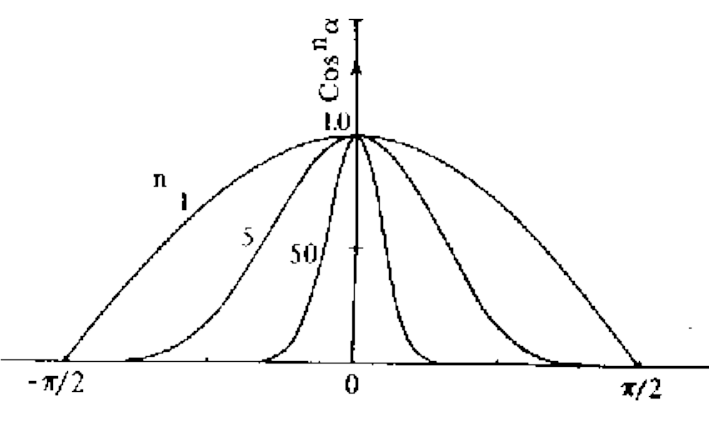
\includegraphics[width=60mm]{pics/cones_of_light.png}}
	\subfigure[]{\label{fig:2lightcones}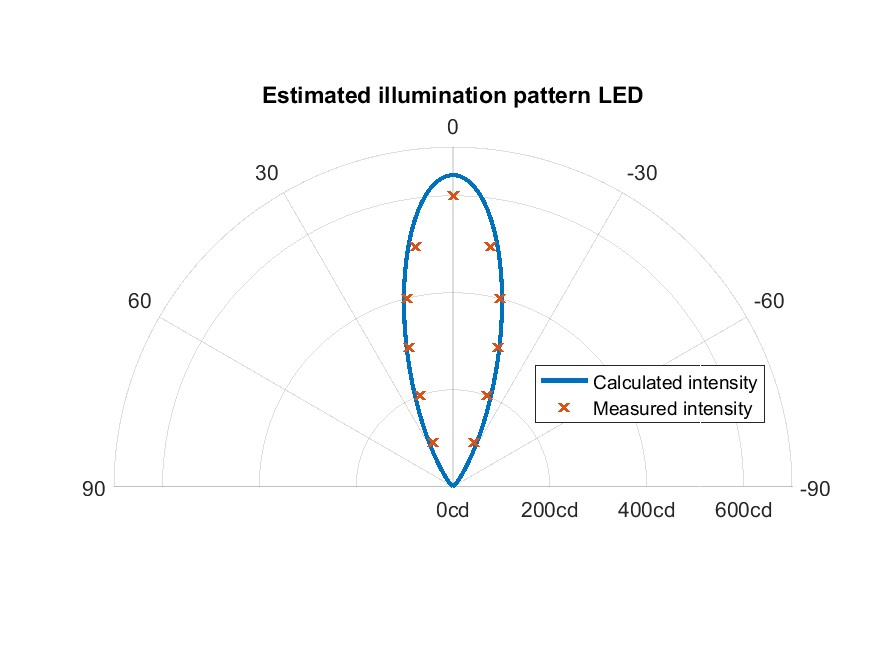
\includegraphics[width=60mm]{pics/polarplot_LED}}
%	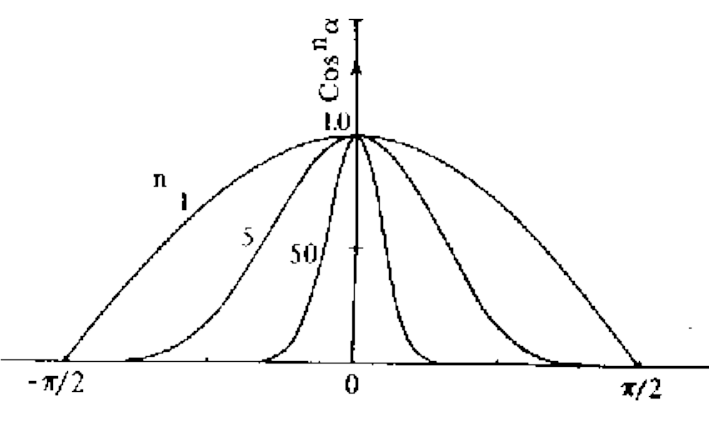
\includegraphics[width=60mm]{pics/cones_of_light.png}
	\caption{(a) shows an overview of how adjusting $\alpha$ changes the light cone of a simulated light source. (b) shows a modelled light cone, modelled with the shown measured light cone.\label{fig:cones_of_light}}
\end{figure}

\subsubsection{Modelling a reflection}
Light impinging on a surface can reflect in three different ways: Diffuse, spread and specular. Almost all surfaces combine several of these reflection types. A visualisation of these reflections can be seen in Figure \ref{fig:phong}.
\begin{figure}
	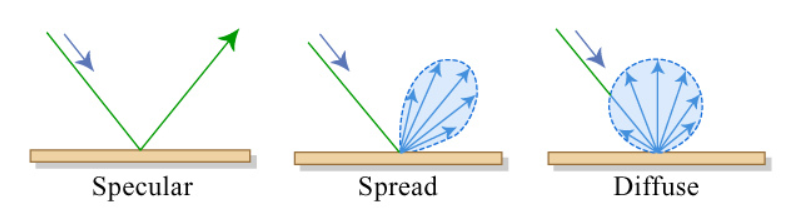
\includegraphics[width=\textwidth]{pics/3_reflections.png}
	\caption{The possible ways for light to reflect when it hits a surface \cite{3reflections}.\label{fig:phong}}
\end{figure}
The \textbf{specular reflection} is a so called perfect reflection. It reflects each incident ray outward, with the reflected ray having the same exit angle to the normal vector $N$ as the incident ray. A material with this kind of property is a mirror. The \textbf{diffuse reflection} is the opposite. Instead of reflecting light in one direction, the light ray is scattered in all directions following a Lambertian emission pattern. This leads to a point, which appears to have the same brightness, no matter the observation angle. A common material with this property is plain white paper. The final kind of reflection is the called the \textbf{spread reflection}. It's a scattered reflection, aimed in the direction of the ideal reflection. A material which has mainly this kind of reflection is matte aluminium.

All of these reflections can be modelled with the help of equation \ref{eq:Reflection}, where $\phi_2$ represents the observation angle. The first part of the equation calculates how much of the impinging light is reflected off the surface and not converted into heat. This is determined by $A$, which represent the albedo of the observed surface. 

The second part describes the actual reflection of the surface. $\frac{\alpha+1}{2\pi}\cos^\alpha(\theta_1'-\phi_2)$ describes the spread reflection and is modelled as light source pointing in the direction of the ideal reflection $\theta_1'$ (see equation \ref{eq:I(phi)}). The higher $\alpha$ is chosen, the more focused the reflection. If $\alpha$ is chosen to be infinite, the surface is modelled as a mirror instead.

$\frac{1}{\pi}\cos(\phi_2)$ describes the diffuse part of the equation and is also modelled with \ref{eq:I(phi)} where $\alpha = 1$. This results in a diffuse reflection. The final term of the equation is $r_d$. This value represents the ratio between the diffuse and spread reflection.

\begin{equation}
\label{eq:Reflection}
R(\theta_2) = E_{hor}\rho(\lambda)\left[ r_{d} \frac{1}{\pi}\cos(\phi_2)+ (1-r_{d})\frac{\alpha+1}{2\pi}\cos^\alpha(\theta_1'-\phi_2) \right]
\end{equation}

\subsubsection{Modelling a photo diode}
The final part missing in the model is the observer. The observer, or receiver in our case, is a photo diode which can be modelled with the help of Equation \ref{eq:receiver_PD}. This equation is very similar to equation \ref{eq:E_hor}, but has one major difference: The $rec(x)$ function. This function checks if the light incoming at angle $\theta_2$ lies in the field of view of the photo diode. If it is, then $rec \left(\frac{\theta_2}{FOV}\right)$ returns 1, otherwise it's 0 and the ray of light wont be counted.

\begin{equation}
	\label{eq:receiver_PD}
	PD = \frac{I\cos(\theta_2)}{d^2} rec \left(\frac{\theta_2}{FOV}\right)
	\qquad
	rec(x) = 
		\begin{cases}
		1, |x|\leq 1 \\
		0, |x| > 1 \\
		\end{cases}
\end{equation}

\subsubsection{Creating a 3D model}
All equations shown in the previous sections can be combined into one big equation, calculating how much a point on the wall is illuminated, reflected and perceived by the observer. This equation is \ref{eq:fullmodel}. It has however a lot of variables, which will make it hard to create a proper simulation. 

\begin{equation}
	\label{eq:fullmodel}
	PD_{tot} = I(\phi,\alpha_{light},\Phi_{lum}) R(\theta_1,\phi_2,\lambda,r_d,\alpha_{floor}) PD(\theta_2,d_2)
\end{equation}
This can be solved by making the problem concrete and simulate it in a 3D space with an $xyz$ coordinate system. If we assume the floor is a plane spanning x and y (thus z = 0) and fix the positions and normals of the LED and photo diode, we can express all angles and distances as formulas of x,y and z. If we then want to calculate total amount of energy perceived by the photo diode, all we need to do is integrate over all the points of the floor (the xy plane).
\begin{equation}
\label{eq:fullmodel_xy}
PD_{tot} = \int_x \int_y I(x,y,z,\alpha_{light},\Phi_{lum}) R(x,y,z,\lambda,r_d,\alpha_{floor}) PD(x,y,z)
\end{equation}

This model was used to create the model used in chapter \ref{Model}. That chapter will also explain what changes were made to obtain the presented model.
\section{Related Work}
\label{sec:Related Work}
This section presents the related work of this thesis. It starts with giving a short overview of several methods used for passive localisation. It shows the projects which use visible light in their localisation schemes. This section finalises by highlighting a paper which attempts to reduce the visible light used in a similar way to this thesis.

\subsection{Passive localisation}
Passive localisation is a hot topic in research and has been tackled by many different research groups in several different ways. The most common method found in literature to detect and track humans is by using Passive Infra-Red (PIR) sensors. These sensors detect the infra-red (heat) radiating from objects and draw conclusions from the observed signals. The passive infrared sensor has been around since 1982 \cite{galvin1982passive} and has been used to detect humans since 1994 \cite{fukuda1994human}.

These days, the research in PIR sensors for detecting and tracking humans focuses in two directions. The first direction is to get more information out of PIR sensors by examining the raw data. M. Waelchli \textit{et al.} for example created a method for estimating the location of a person within the view of the sensor \cite{PIR_Single_Tracking}. The second direction is to track humans with the help of several linked sensors. An example of this, by P. Zappi \textit{et al.} is \cite{PIR_Tracking}. They linked a server to multiple binary human activity sensors, in order to locate and track humans in an indoor building.

Another method for passive localisation, which popped into existence more recently, is developed by M. Youssef \textit{et al.}\cite{WIFI_Tracking}. They created a detect and track application with the help of WIFI access-points (APs), WIFI monitoring-points (MPs) and an application server (AS). The MPs measure the signal strength of the APs, and transmit this data to the AS. The server runs a moving variance algorithm on all of the received signals to detect significant changes in the signal. An overview of the complete system can be seen in figure \ref{fig:WIFI-tracking}.
\begin{figure}[]
	\centering
	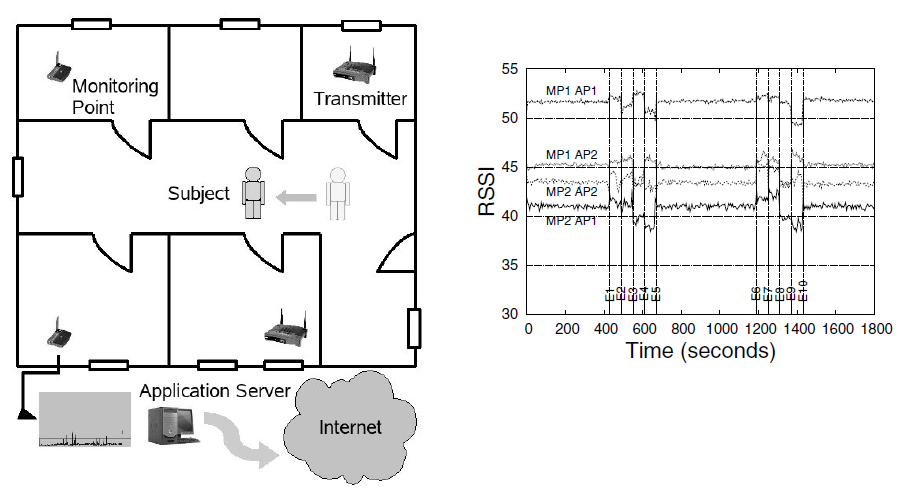
\includegraphics[width=\textwidth]{pics/MovingVarriance1.png}
	\caption{Overview of the WIFI tracking system of Moustsafa Youssef \textit{et al.} \cite{WIFI_Tracking}. The left figure shows an overview of the setup where the right figure shows the strength of the APs from the point of view of the MPs. E1 to E8 represent possible 'events' of bypassing persons.\label{fig:WIFI-tracking}}
\end{figure}

Another approach to passive localisation is to use the tiles upon we walk as sensors. This was done by M. Valtonen \textit{et al.} \cite{Tile_Track}. The system measures the capacity between several floor tiles and a receiving electrode. With the help of the measurements, they estimate the position of the person standing on top of the tiles.

\subsection{Passive Visible Light Localisation}
In recent years, a new method for locating and tracking humans has been explored: Passive Visible Light Localisation (PVLL). This method is focussed on using visible light and photo sensors to detect and track humans and objects. Several of these project will be explained briefly, followed by a short comparison between these projects and Dark Sensing.

\subsubsection{Local Light}
Local light, developed by Lascio \textit{et al.}\cite{LocaLight}, is a system which implements passive localization with the help of visible light. The system consists of 3 parts. A light, light sensing RFID tags and a server. The light illuminates the environment. The RFID tags are mounted in the floor, detecting the light produced by the luminaire. The tags transmit their data to a server which processes the data. An overview of the system can be seen in Figure \ref{fig:LocalLight}.

The system works by detecting changes in the light intensity. If the photo diode suddenly senses a huge drop in light, because a shadow is casted on the photo diode by an object or person, the system triggers a detection. The server knows the exact location of all luminaries and photo diodes and is therefore capable to of determining where the object or person is at this moment in time.

\begin{figure}[]
	\centering
	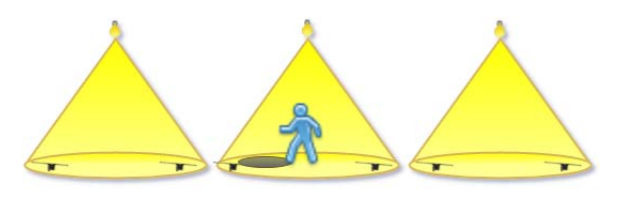
\includegraphics[width=90mm]{pics/LocalLight.png}
	\caption{Overview of the LocalLight system of E.D. Lascio \textit{et al.}\cite{LocaLight}. Lights on the ceiling and light sensing RFID tags on the floor.\label{fig:LocalLight}}
\end{figure}

\subsubsection{Activity sensing using ceiling photo diodes}
Two different projects have been found which have develop a passive localisation scheme using several light/photo diode pairs mounted together on the ceiling. Both take a slightly different approach.

The first project, by J. Zhang \cite{JakesWork}, created a method capable of localising objects on a line between two light/photo diode pairs. By moving an object with three reflective surfaces underneath a light, he managed to localise them at several points on the line by using the specular component of the reflections bouncing of the object. His test set-up can be seen in figure \ref{Zhangpicca}.
\begin{figure}[]
	\centering
	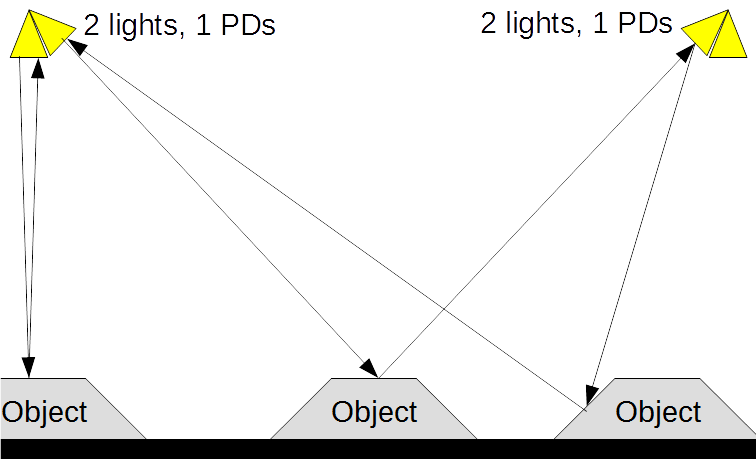
\includegraphics[width=90mm]{pics/Pic_Jake.png}
	\caption{Overview of the system used by J. Zhang \cite{JakesWork}\label{Zhangpicca}}
\end{figure}

The other project, by M. Ibrahim \textit{et al.}, makes use of modulated lights. Each luminaire transmits light in a different pattern. The photo diode, which is placed next to the light, detects what patterns of light it perceives. If the photo diode does not sense one of the lights it normally does, it triggers a detection as the light was intercepted by a bypassing object. An overview of the set-up can be seen in Figure \ref{fig:Ceiling_PD}

\begin{figure}[]
	\centering
	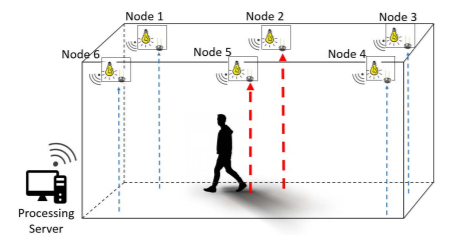
\includegraphics[width=90mm]{pics/lightspdceiling.png}
	\caption{Overview of the system set-up used by M. Ibrahim\cite{Ceiling_PD}. In this specific situation node 2 and 5 detect no light from node 1, because a person is blocking the light.\label{fig:Ceiling_PD}}
\end{figure}

\subsubsection{Comparison with Dark Sensing}
The Dark Sensing project differs from the existing projects in several ways. It's the only project tempting to create a sensing device, only requiring one sensor node instead of multiple and is therefore easier to install and expand. It's also the only project which attempts to detect humans with the main drive of saving energy. It's also the only project which potentially can be implemented outdoor, mounted on a light post for example, as the other PVLL projects where require either a server in reach of the sensors, or other specific environmental features. Dark Sensing has the potential to be a stand alone product.

The downside of Dark Sensing is that it only focuses on detecting activity. It's therefore unable to determine where the activity is exactly. All of the other projects are way better in that specific area.

\subsection{Other related projects}
One project which has nothing to do with passive localisation, but can't miss from the related work section is \textit{"The dark light rises"} by Z. Tian \textit{et al.} \cite{Dark_Light_Rises} \cite{Dark_VLC}. This group explores the idea of Visible Light Communication (VLC) with dark light, a VLC primitive that allows light-based communication to be sustained even when LEDs emit extremely-low luminance. The communication works by generating high power, but short light pulses (500ns). These pulses are then used in a pulse position modulation scheme to achieve communication (1.8Kbps at 1.3m) with light while being nearly invisible to the end user. The goals of Dark sensing and Dark VLC are similar: Save light and therefore energy. Both projects however apply this method in other applications.
\chapter{Model}
\label{Model}


A model has been made with two goal of answering two questions:
\begin{enumerate}\itemsep2pt
	\item How strong are the reflections of flashes in a realistic environment?
	\item How much will these reflections change if an object enters the illuminated area
\end{enumerate}
This section describes how the model explained in section \ref{sec:Characteristics of light} was adjusted and implemented to answer the questions posed above

\section{Model description}
The model made is an interpretation of the phong reflection model (see section \ref{sec:Characteristics of light}). It calculates how much of the light leaving a luminaire, bounces back via the environment to a photodiode placed next to the light source. This section will first discuss the adjustments made to the phong model, followed by an explanation of the calculation process.

\subsection{Adjustments}
The first adjustment is the removal of "time". The methods in the literature took the travelling time of light into account in order to calculate the possible inter-symbol interference. This is not required for this simulation as we are only interested in the steady state situation when the light is fully turned on and the light received by the photodiode is maximized for the current situation.

The second adjustment is the removal of "colour". The original method differentiated between different wavelengths of visible light when reflecting light of off surfaces and was therefore maintaining colour information. This is however not necessary for this model, as we do not care about the colour of the reflecting objects, but only about the total amount of energy reflected by the object. For this reason, the surface reflection coefficient ($p(\lambda)$) was replaced with the albedo of the object instead.

Albedo is a property of an object representing the percentage of energy which is reflected when sun is shining on the object. Even though albedo is based on the full spectrum of sunlight instead of only the wavelengths of visible light, it gives a reasonable approximation of the reflection coefficient in this scenario. This will be shown in section \ref{sec:verification}.

\begin{equation}
\Gamma = \int_{380nm}^{780nm} \Phi_e p(\lambda) d\lambda \to \Gamma = \Phi_{lum} \alpha
\end{equation}

The final adjustment is the amount of reflections we calculate. In reality a light ray can be reflected an infinite amount of times of several different surfaces before returning back to the sensor. In the model however we only calculated one bounce (from the light to an object and back) for two reasons. The reason for this is that the first reflection provides approximately 80\% of the signal where all other reflections only make up 20\% of the total power\cite{indoor_VLC_no_LOS}. This increase in accuracy

\begin{equation}
\label{eq:Ehor_new}
E_{hor}=\frac{I(\phi)\cos(\varphi)}{d^2}=\frac{I(0) cos^m(\phi)\cos(\varphi)}{d^2}
\end{equation}

\subsection{Calculation process}
Calculating the amount of light reflecting back to the object is a three step process. The first step is to calculate the shadow casted by the object on the floor and walls. This is required as the surface where the shadow is casted can't reflect light back directly to the photo diode. It's important to note that light casting the shadow is reflected of the object instead and with that, changes the reflection pattern of the room.

The second step is to calculate how much light reflected from all floors and walls (where no shadow is casted) to the photo diode. The finals step is to calculate how much light is reflected from each side of the object. \ref{fig:raytracing} shows an overview of an environment with rays leaving the light, casting shadow and the resulting reflections.

\begin{figure}
	\centering     %%% not \center
	\label{fig:raytracing}
	\subfigure[Sideview]{\label{fig:a}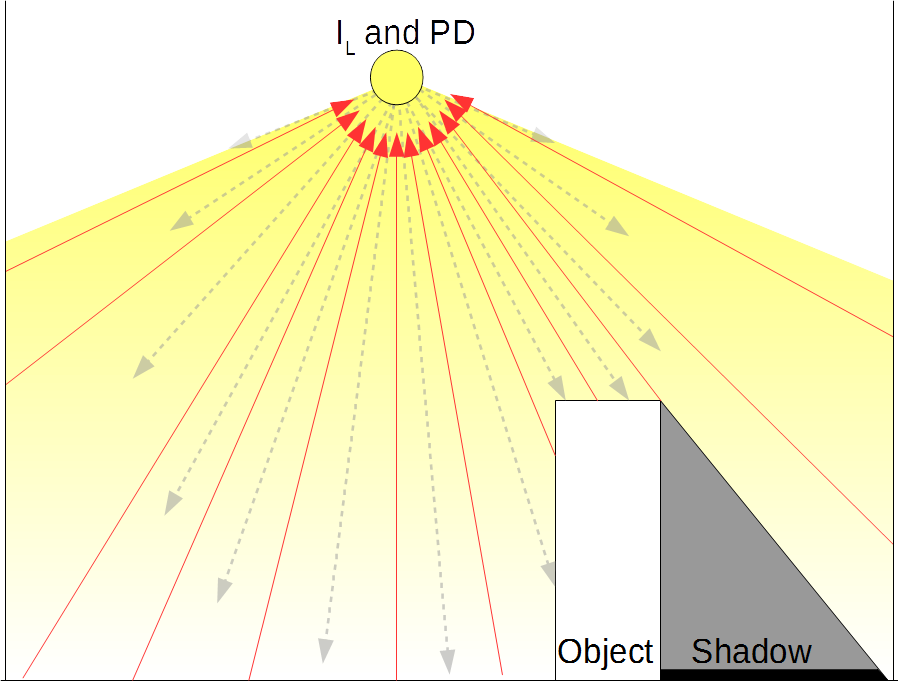
\includegraphics[width=68mm]{pics/Calculation_frontview.png}}
	\subfigure[Topview]{\label{fig:b}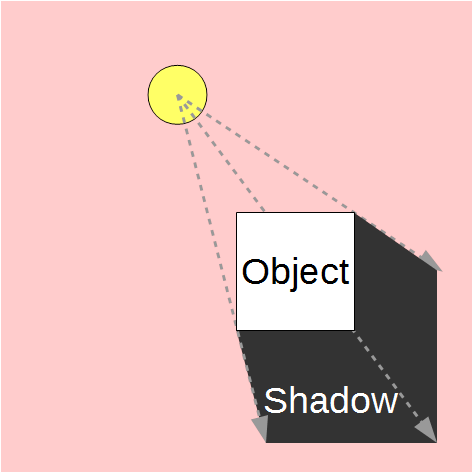
\includegraphics[width=52mm]{pics/Calulation_topview.png}}
	\caption{Overview of the calculation process. Grey lines represent light rays casted by the light. Black represents the shadow casted by the object on the floor or walls. Red lines or areas show reflections bouncing from the ground, walls or object back to the photo diode.}
\end{figure}

\section{Verification}
\label{sec:verification}
The calculation method was verified using a scale model featuring a LED\cite{lamptest}, a paper box and a light meter\cite{LuxMeter}. The first step of verifying the model is check if the LED is modelled properly. This was done by hanging the LED at 100cm above the floor and measuring the horizontal illuminance ($E_hor$) at the floor to see if the measured irradiation pattern of the LED matches the theoretical pattern produced by equation \ref{eq:I(phi)}. Simulations in Appendix \ref{app_repository} that the LED in the test set-up was producing more light than in the specification.

The second step is the verification of the interpretation of the Phong model. This was done with the test set-up shown in figure \ref{fig:VerificationSetup}. By moving a paper box across the flool in steps of 5cm and measuring the reflection at each step we obtain the red line in figure \ref{fig:verf_floor}.

\begin{figure}[]
	\centering
	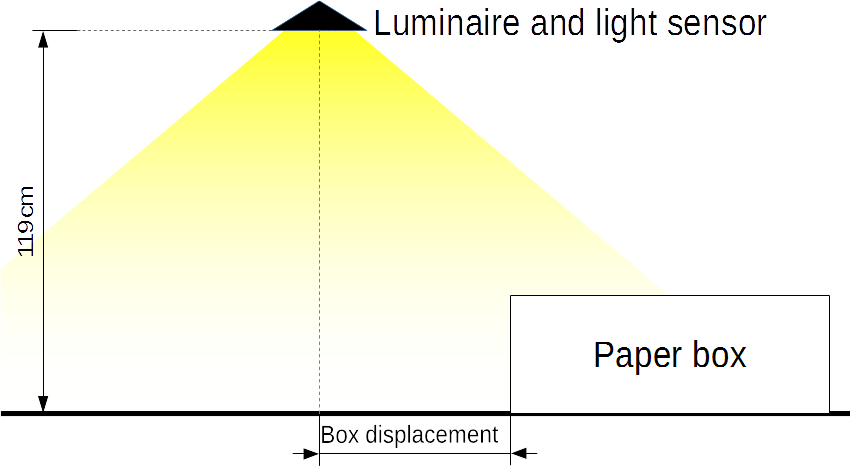
\includegraphics[width=\textwidth]{pics/Verification_Situation.png}
	\caption{Visualisation of the model verification set-up.}
	\label{fig:VerificationSetup}
\end{figure}

\begin{figure}
	\centering     %%% not \center
	\label{fig:VerificationResults}
	\subfigure[]{\label{fig:verf_paper}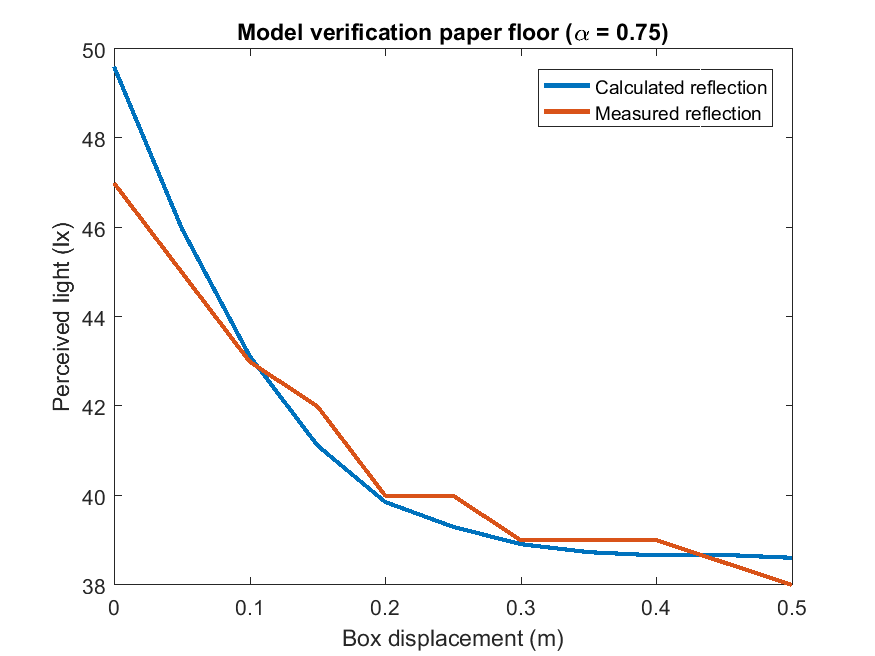
\includegraphics[width=60mm]{pics/ModelVerificationResults_paper.png}}
	\subfigure[]{\label{fig:verf_floor}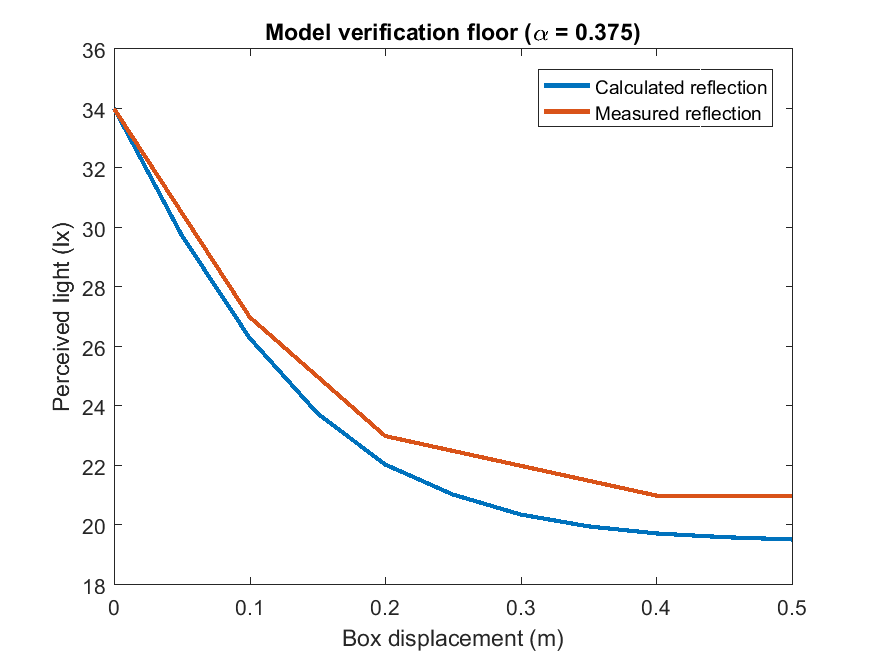
\includegraphics[width=60mm]{pics/ModelVerificationResults_floor.png}}
	\caption{Both figures show that the model provides a reasonable approximation of the reality. Note that the albedo of paper was taken from \cite{Albedo} and the albedo of the floor was estimated with these measurements.}
\end{figure}

\section{Modelling of the hallway}
\label{sec:moddelingofthehallway}
The hallway modelled is based on a real hallway located at the TU Delft. The hallway is 2.2m wide and 2.8m high. The floors albedo is set at 0.37, as this was calculated during the verification of the model. The albedo of the walls was set to 0.95 which represents the albedo of white plaster\cite{Albedo}. The reflection of these surfaces is assumed to be fully diffuse ($r_d = 1$).

Industry standards state that corridors in education buildings should be illuminated with at least $E_{mean} > 100lx$ and a light uniformity of $U_o > 0.4$\cite{lichthandbuch}. These lighting requirements can be achieved using the same luminaire used during the verification process if hung in the staggered formation shown in figure \ref{fig:pattern_hallway}. Calculations showing that the industry standards are met can be found in Appendix \ref{app_repository}.

The object passing by the light (representing a human) will be modelled as a cuboid 0.5m long and 0.2m wide with varying heights. Several albedos have been assigned to the cuboid to represent the different kind of clothing humans wear. The object will be moved in a straight line trough the hallway with the light at a set vertical distance y. Some example paths can be seen in figure \ref{fig:traveling_path}.

\begin{figure}
	\centering     %%% not \center
	\subfigure[Staggerd hallway LED pattern ]{\label{fig:pattern_hallway}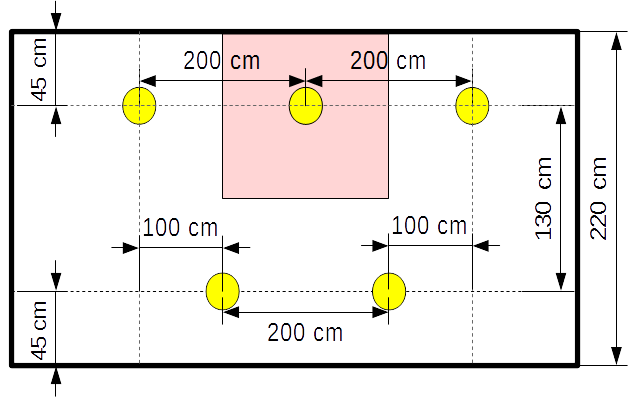
\includegraphics[width=60mm]{pics/LightsOverview.png}}
	\subfigure[Traveling path of the object ]{\label{fig:traveling_path}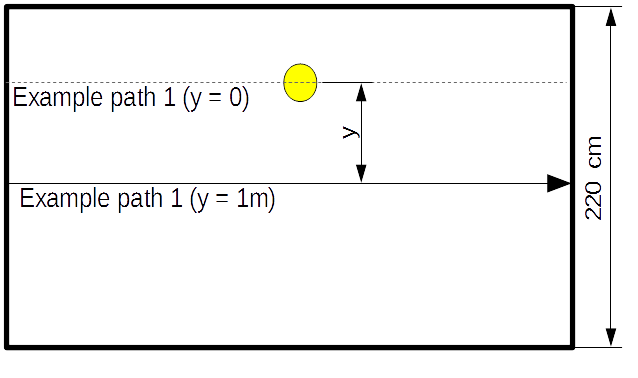
\includegraphics[width=60mm]{pics/TravelingPath.png}}
	\caption{Figure a shows the position of the luminairs to obtain a realistic illumination pattern. Figure b shows an example travelling path of an object.}
\end{figure}

\section{Modelling of the street}
The street model is based on a real street near the TU delft. It has two lanes for a cars (each 3m wide), and sidewalk (2m wide). The albedo of the street will be modeled with different values for old ($\alpha = 0.06$) and new asphalt ($\alpha = 0.14$), as asphalt loses reflectivity if it grows older\cite{Albedo}. The reflections of the street are assumed to be fully diffuse ($r_d = 1$).

Industry standards state that a street with side walk should be illuminated with at least $E_{mean} > 3lx$ and a light uniformity of $U_o > 0.2$ \cite{HandboekBestaandeBouw}.These lighting requirements can be achieved using 700lx luminaires with a halfpower angle of $60^{\circ}$ placed every 15 meter in between the road and side walk. This set-up is visualized in figure \ref{fig:pattern_street}. Calculations showing that the industry standards are met can be found in Appendix \ref{app_repository}.

In this model two different objects will be modelled representing humans (walking on the side walk) and cars (driving in the two driving lanes). The humans will be modelled in the same way as in section \ref{sec:moddelingofthehallway}. The car will be modelled as a cuboid with the dimensions of an Opel Corsa (4m x 1,7m x 1,5m), a commonly seen small car. The object was modelled with diffuse reflection, because no reliable sources describing the specular parameters ($r_d$ and $m$) of cars could be found.

Lacking the specular deflection for this specific model should not influence the results significantly. This is because no part of the car will be moved directly underneath the light and therefore no significant amount of light of the spread reflection should ever reach the light sensor. This is visualized in figure \ref{fig:streetnospecular}. This is also the reason why cars are simulated with lower albedo than humans.

\begin{figure}
	\centering     %%% not \center
	\subfigure[Topview of the street model ]{\label{fig:pattern_street}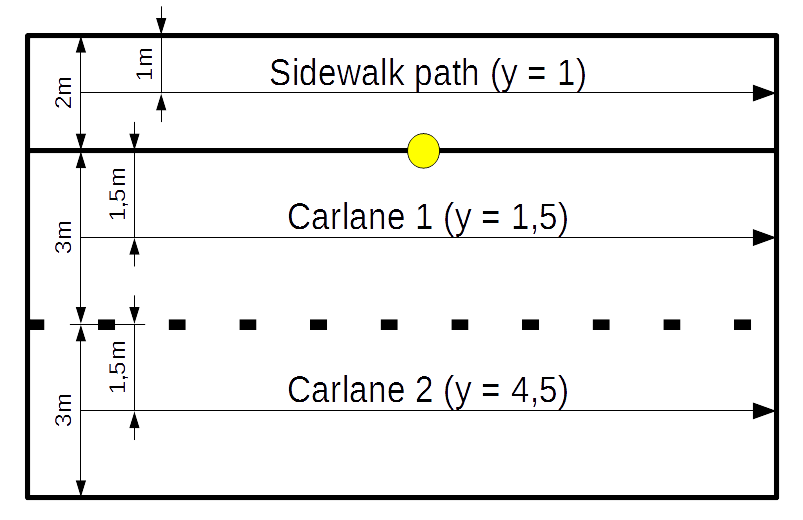
\includegraphics[width=70mm]{pics/TravelingPath_street.png}}
	\subfigure[Spread reflection on cars ]{\label{fig:streetnospecular}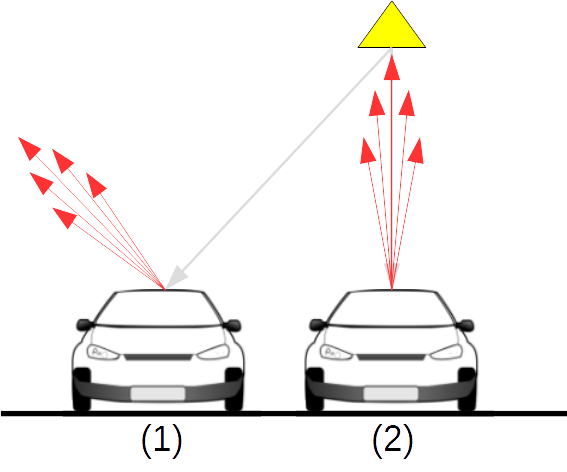
\includegraphics[width=50mm]{pics/StreetNoSpecular.png}}
	\caption{A shows an overview of the model. B shows why the spread reflection component plays no part in this model for cars.}
\end{figure}

\section{Results}
Several measurements have been graphed in Figure X. Raw results can be viewed in appendix \ref{app:RawModelResults}.

%voeg plaatjes toe voor conlusie

\section{Conclusions}

Influence of albedo

approximate the minimum and maximum signal frequency.



\chapter{Platform}
\label{chp:Platform}
A device has been made to generate, receive and analyse flashes. The complete system architecture is shown in figure \ref{fig:systemOveriew}. Each component and their interfaces will be discussed briefly, followed by a section describing the final build of the platform.

\begin{figure}[h]
	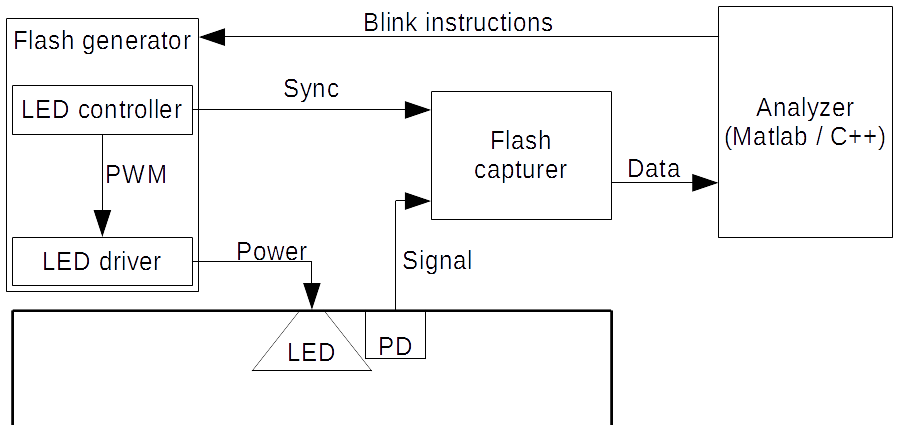
\includegraphics[width=\textwidth]{pics/systemOverview.png}
	\caption{System architecture of the flash generator/analyser.\label{fig:systemOveriew}}
	
\end{figure}

\section{system components}

\subsection{Flash generator}
The flash generator is a device able to control a LED with high precision. It's able to set the period $T$, and the t-on time $T_{on}$. $T$ Controls the frequency of the flashes and $T_{on}$ length. Both parameters can be set with a resolution of $10\mu s$ resulting in a precisely controlled PWM signal with the help of equation \ref{eq:1/f=T}. This signal is sent to a LED driver trough one of three LED drivers, which will make the actual light turn on and off at different light levels.

\begin{equation}
\label{eq:1/f=T}
T=\frac{1}{f}
\qquad
DutyCycle=\frac{T_{on}}{T} * 100\%
\end{equation}
Besides generating the PWM signal for the light, the flash generator has another function. It sends a sync signal to the flash receiver just before generating a flash. This allows the flash generator to be ready when the flash starts, so it does not waste time sampling if no flash is generated.

\begin{figure}[]
	\centering
	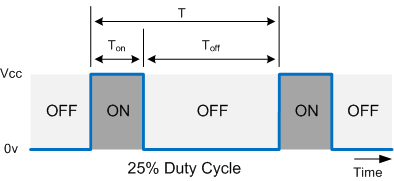
\includegraphics[]{pics/DutyCycle.png}
	\caption{Visualization of how $T$ and $T_{on}$ determine the duty cycle and frequency of the flash generator.\label{fig:DutyCycle}}
\end{figure}

\subsection{Reflection receiver}
The job of the receiver is to sample values while the light is being turned on and off, to then analyse the full reflected flash and extract a feature which properly represents the environment. The receiver should therefore capture flashes as precise and consistent as possible. For this reason, the receiver receives a sync signal from the flash generator and is therefore able to start sampling at almost the same moment every time, relative to the start of the flash. 

The receiver should continue sampling for a set period of time. Once done, the device should do one of the following things with the received samples, depending on the mode of the analyser:
\begin{enumerate}[itemsep=-1ex,topsep=0pt]
	\item Send back the full flash, uncompressed, for the analysis of separate flashes.
	\item Send back all compressed flashes, by extracting several features.
\end{enumerate}

\subsection{Analyser}
The analyser will receive samples from the reflection receiver and is ran on a PC in the form of either a C/C++ program (real-time) or as a MATLAB script (post-time). The analyser can set the receiver to raw or compressed mode. If the receiver sends raw flashes to the analyser it can be used to analyse these flashes. This mode is used in chapter \ref{chp:Flash_Analysis} to analyse single flashes in order to find the ideal settings for the flash generator and reflection receiver. If the receiver sends compressed flashes, the analyser is able to analyse consecutive flashes. This mode will be used in chapter \ref{chp:Analyser} to find an algorithm to determine if an object is moving in the area under the light.

The Analyser should also be able to control the flash generator if the system is running in real-time mode. It is therefore able to send a packet with $T$, ${T_{on}}$ and $I_{LED}$ to the device. This allows for real time control of the flash generator.

\section{Implementation}
The system was build by combining several of shelve parts. An overview of the actual build can be seen in figure \ref{fig:acutalBuild}. It shows the different components mounted on a box. This section will explain briefly how each system component is implemented and why each part was chosen.

The flash generator is implemented on an Arduino UNO\cite{ArduinoUno}. This platform was chosen, as it's simple to use, does not require an operating system (OS) and has therefore no unexpected jitter. The LED used in the set-up is the same LED as modelled in chapter\ref{Model}. The power used by the LED is regulated with a single resistor. The resistors where chosen after some experimentation with the flash generation and reception. The values and resulting LED current can be seen in equation \ref{eq:Power}.

\begin{equation}
\label{eq:Power}
I_{LED}=\frac{V_{DD} - U_{LED}}{R}
\qquad
I_{LED} = \frac{7 - 3.6}{[1, 3, 5]} = [3.4A, 1.1A, 0.68A]
\end{equation}

The reflection receiver is implemented on the shine platform \cite{Shine}. This platform was chosen because it's a simple (no OS required) hands-on platform featuring multiple photo diodes by default. The original software of shine sampled each photo diode at 1Khz. This is way too low to see the $10\mu s$ flash resolution. For this reason the software of shine was rewritten to sample in bursts of 50 samples at 210Khz (for a total of$\pm 240\mu s$) when the sync signal is received.

A downside of the shine platform is that it's unable to communicate directly with the analyser as it does not has a FTDI interface. This problem was solved by using a processor-less Arduino UNO as bridge between the analyser and shine platform.

The receiver makes use of three photo diodes. The original sensors on shine where replaced with ones more sensitive to visible light. Each sensor is also configured in a different way. Some feature an increased amplification of the measured signal. Others have a longer wire with (intentional) bad shielding which can simulate how the system preforms in a environment with lots of electromagnetic radiation. An overview of the PD configurations can be seen in table \ref{tbl:PDs}.

Another important decision concerns the amplification circuit of the photo diode. The original circuit used by shine features an analogue low-pass filter to remove ripple introduced by the amplifier (See Figure \ref{fig:FristFlashes}). The filter has several side effects. It reduces the signal strength and decreases the time the signal is visible to the system. It was therefore chosen to remove al analogue filters from shine and deal with the ripple with the help of software if required. The ripple effect might even be useful as the it's probably dependent on the received signal and therefore a measure of light the environment.

\begin{table}[]
	\centering
	\begin{tabular}{clll}
		PD\#                   & Wire length & Gain  & EMC Shield \\ \cline{2-4} 
		\multicolumn{1}{c|}{1} & Long        & 1000  & Slecteable \\
		\multicolumn{1}{c|}{2} & Short       & 5600  & Yes        \\
		\multicolumn{1}{c|}{3} & Short       & 10000 & Yes       
	\end{tabular}
	\caption{Overview of photo diode configurations.\label{tbl:PDs}}
\end{table}

\begin{figure}
	\centering     %%% not \center
	\subfigure[Top view]{\label{fig:top}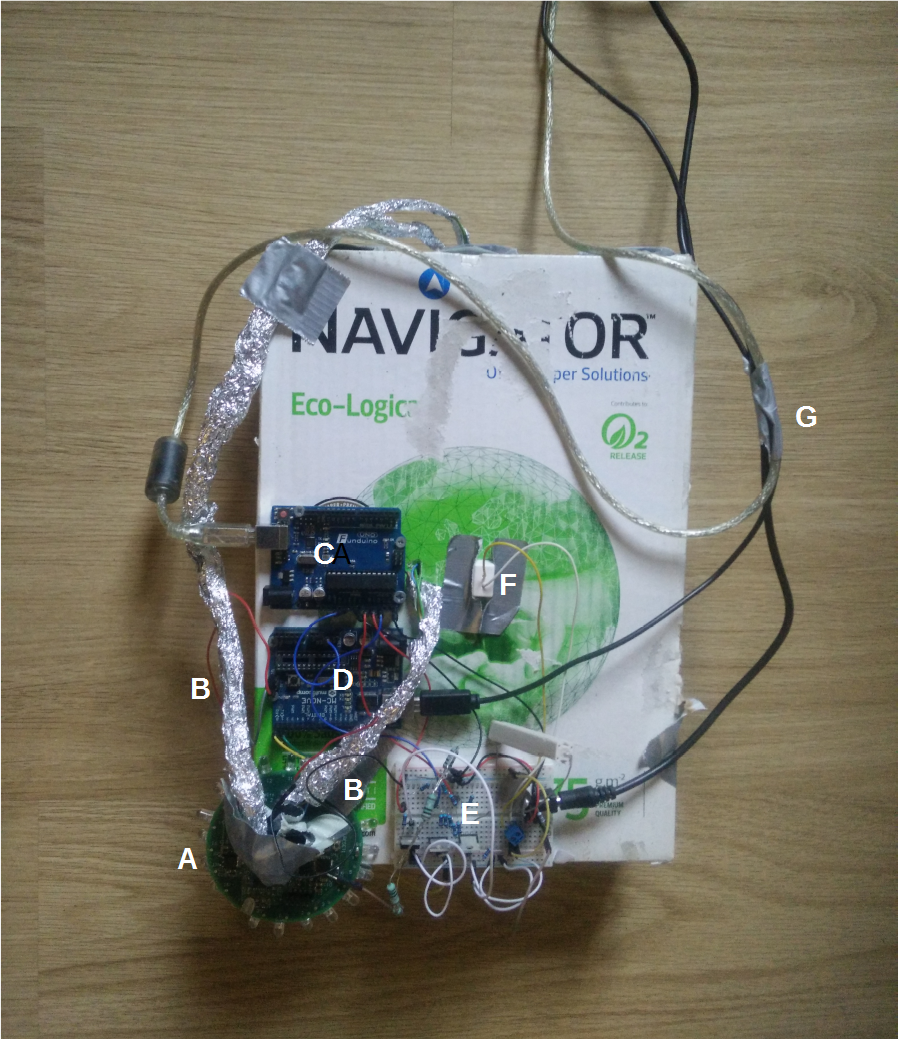
\includegraphics[width=60mm]{pics/platform_top.png}}
	\subfigure[Bottom view]{\label{fig:bot}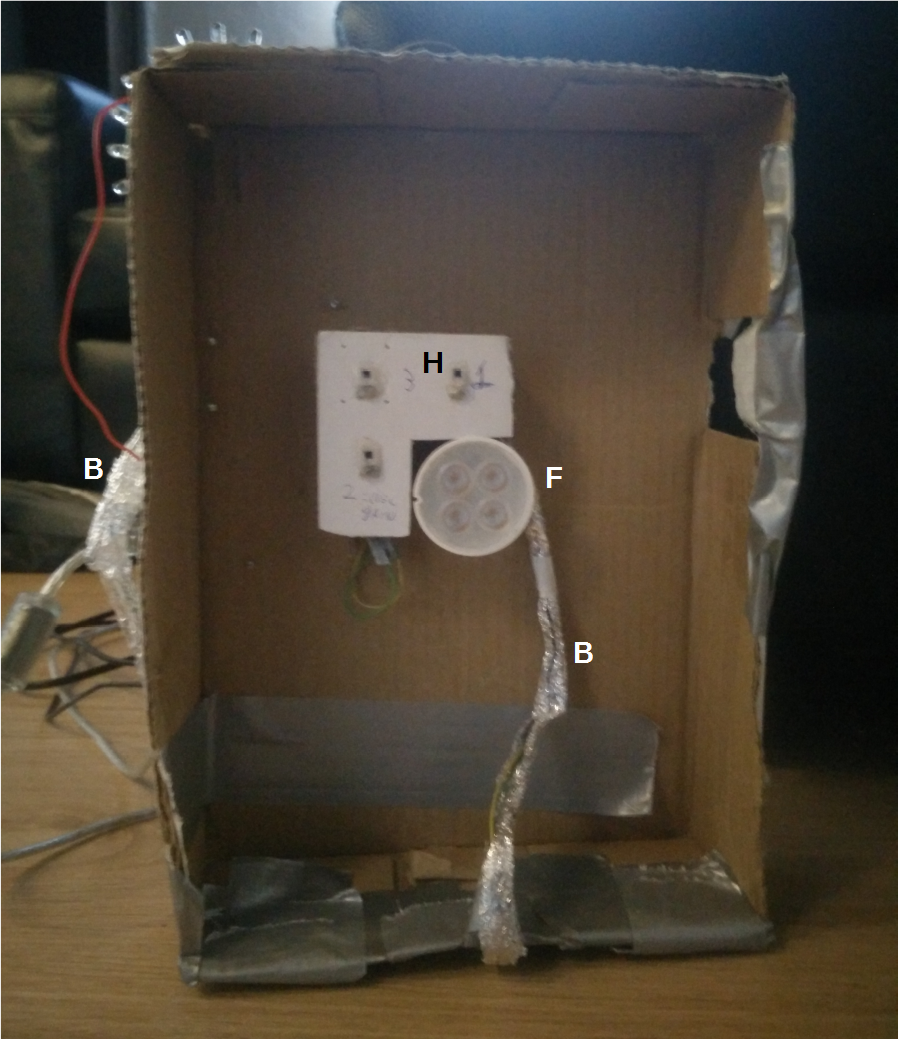
\includegraphics[width=60mm]{pics/platform_bot.png}}
	\captionsetup{singlelinecheck=off}
	\caption[]{The platform prototype. Each letter denotes a different component:
		\begin{enumerate}[label=\Alph*,itemsep=-1ex,topsep=0pt]
			\item = Reflection receiver
			\item = Wires to the photo diodes
			\item = LED controller
			\item = Communication bridge between shine and the PC
			\item = LED driver
			\item = The LED
			\item = Wires to the analyser and power supply
			\item = Three photo diodes
	    \end{enumerate}\label{fig:acutalBuild}}
\end{figure}

\section{Evaluation}
The system has been build and tested. Even though the created device has a poor build quality, it has great potential for experimentation with the proposed method of activity detection. The main advantages are:
\begin{itemize}[itemsep=-1ex]
	\item Each building block has one clear purpose and can therefore be tackled separately from other components. It's therefore impossible that a timing error in the flash generator software affects the sampling of the receiver or vice versa.
	\item The build quality is poor. If the project works on this device, it will definitely work on a dedicated platform.
\end{itemize}
The next steps for the project is finding a method for extracting useful information from flashes as shown in figure \ref{fig:notfiltered}. 

\begin{figure}
	\centering     %%% not \center
	\subfigure[Unfiltered flash]{\label{fig:notfiltered}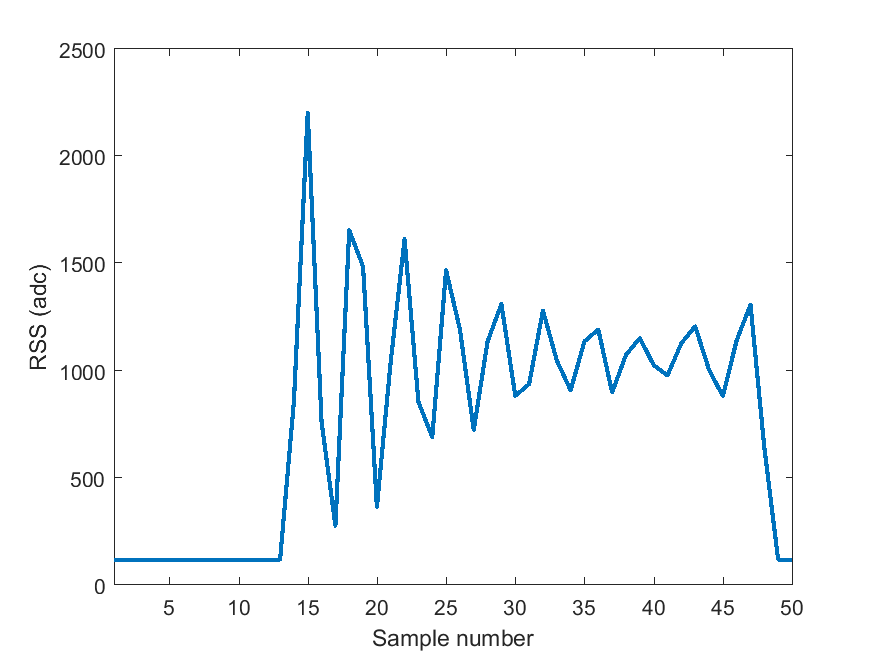
\includegraphics[width=60mm]{pics/no_filter.png}}
	\subfigure[Filtered flash]{\label{fig:filtered}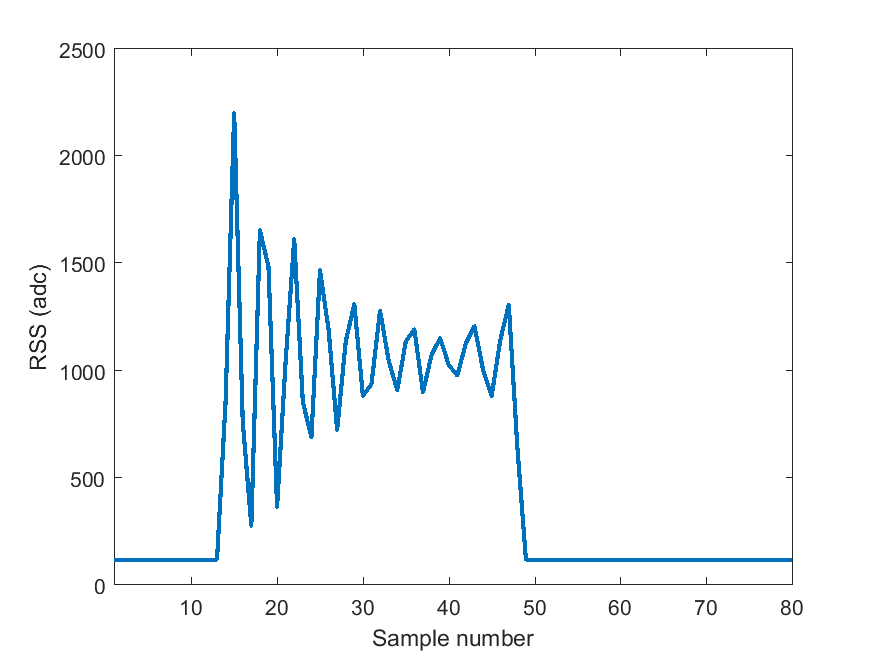
\includegraphics[width=60mm]{pics/analog_filter.png}}
	\caption{Two flashes captured with the platform. Left is unfiltered, right is filtered.	\label{fig:FristFlashes}}
\end{figure}
\chapter{Flash Analysis}
\label{chp:Flash_Analysis}

%checklist:
% - introduction (goal)
% - Test setup
% - Proceedings in this chapter

The goal of this chapter is to find a method, capable of obtaining consistent measures of the environment from measured flashes. Secondary goals are to achieve this with the shortest flash and while using a small amount of computation power.

In this chapter, the platform is set-up as seen in figure \ref{fig:Flashcapturing}. 
D in the figure represents the distance between the device and the reflecting surface (the floor in this case). All measurements presented in this chapter have been made in a darkroom, a room where no lights from outside can enter, so the test result won't get influenced by other illumination sources.
 
The set-up will first be used to get a reasonable understanding of what flashes look like and how settings of the flash generator influence the received flash. Then, several methods for obtaining a measure of the environment from flashes will be presented and compared. This chapter will conclude with the final settings used in the flash generator and an algorithm to obtain a consistent measure of the environment from the received flash.
\begin{figure}
	\centering     %%% not \center
	\subfigure[Test setup in illuminated environment]{\label{fig:Flashcapture_light}\includegraphics[width=60mm]{pics/Flashcapture_light.png}}
	\subfigure[Test set-up in dark environment]{\label{fig:Flashcapture_dark}\includegraphics[width=60mm]{pics/Flashcapture_dark.png}}
	\caption{Test set-up used to capture flashes in the darkroom.\label{fig:Flashcapturing}}
\end{figure}

\section{Flash properties}
\label{sec:Flash_generator}
The test set-up has several parameters which can affect the perceived flash: $T_{on}$ (on time of the LED), $I$ (brightness of the LED), $PD$ (sensitivity of the photo diode) and $D$ (distance between device and reflecting surface). This section shows how each of these parameters influences the received signal. Note that the period, $T$, is not present in the list as should not influence an individual flash.

Figure \ref{fig:InfOfTon} shows several responses for different $T_{on}$. The figure shows that all signals closely match each other, until the light is turned off. This is a useful property as this means it's possible to reduce the $T_{on}$ with no influence on the signal, if the ending of the flash is not used.

Figure \ref{fig:InfOfI} shows the influence of using the different amplification circuits of the flash generator. It can be seen that the LED powered with the lower resistance (and thus a higher LED current) is perceived as brighter to the system than the lights powered with a bigger resistor. It's also observed that the LED powered with higher currents show up earlier to the system. This is because LEDs driven with higher currents turn on faster \cite{LED_on}. This means that if a lower LED current is used a bigger $T_on$ is required to obtain useful information.

Figure \ref{fig:InfOfD} shows a set of measured flashes at a variance distance from the wall. It clearly shows that if the distance increases, the observed light decreases. This is logical, as when light travels longer distances, the relative intensity of the light decreases. 

Figure \ref{fig:InfOfPD} shows what happens when the different photo diodes are used. As expected, the RSS rises once we increase the gain on the photo diode. $PD_3$ almost instantly saturates as the gain is too strong when used in combination with $I_1$. $PD_3$ is therefore also displayed with in combination with $I_3$. Another noticeable change is the ripple frequency caused by the amplifier This change is expected, as the resistor in the feedback loop of the amplifier was changed.

\begin{figure}
	\centering     %%% not \center
	\subfigure[]{\label{fig:InfOfTon}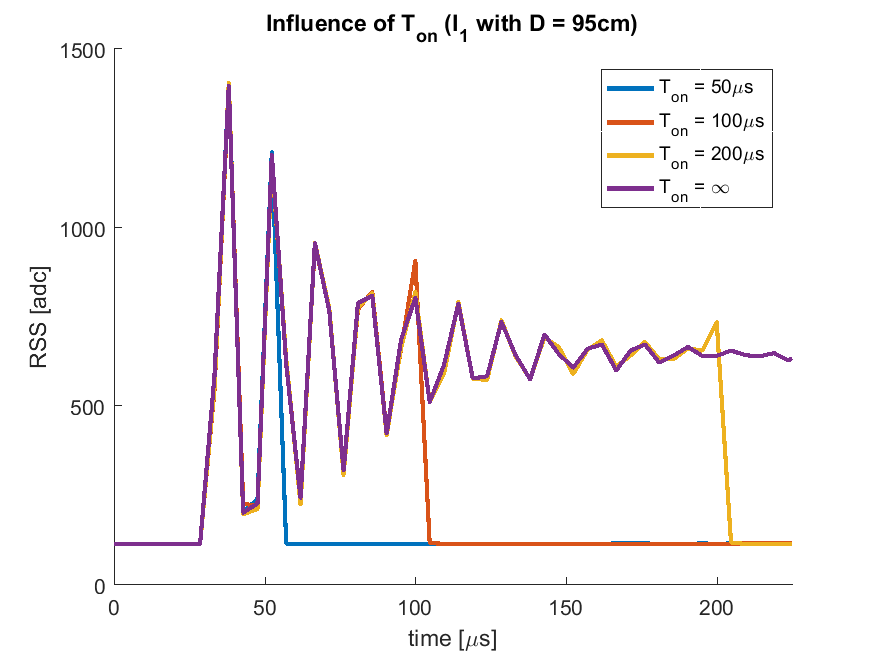
\includegraphics[width=60mm]{pics/InfluenceOfTon.png}}
	\subfigure[]{\label{fig:InfOfI}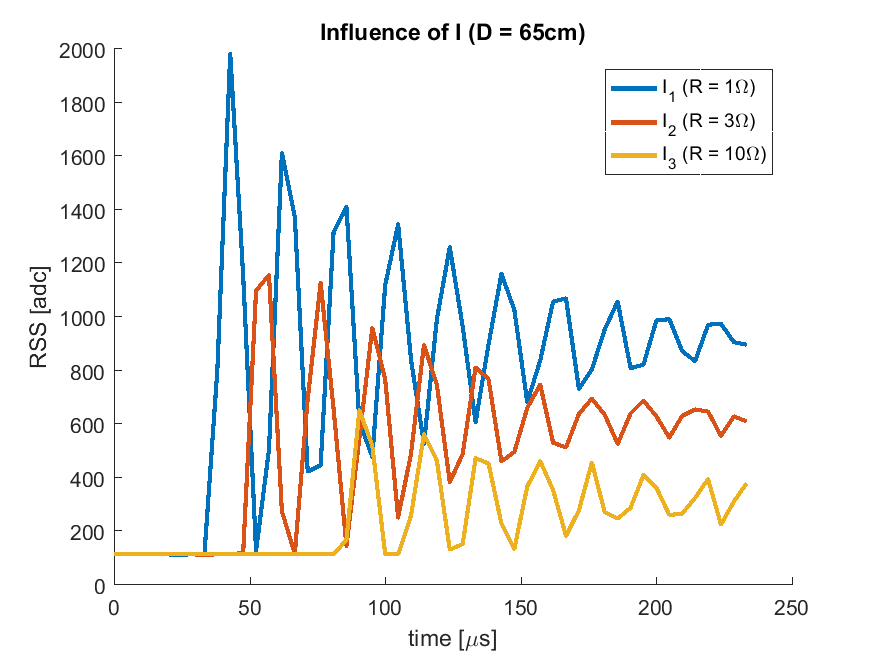
\includegraphics[width=60mm]{pics/InfluenceOfI.png}}
	\\
	\subfigure[]{\label{fig:InfOfD}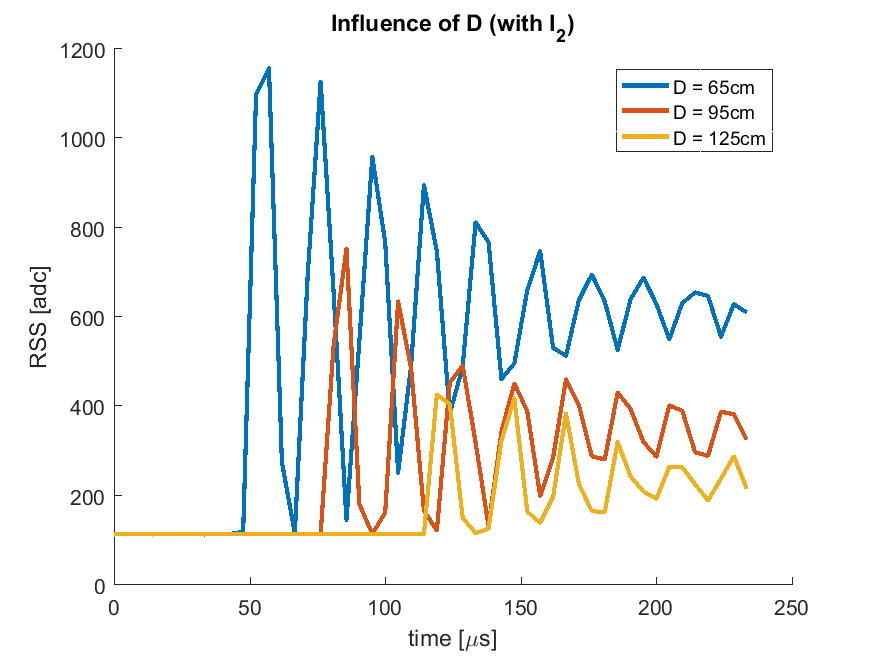
\includegraphics[width=60mm]{pics/InfluenceOfD.png}}
	\subfigure[]{\label{fig:InfOfPD}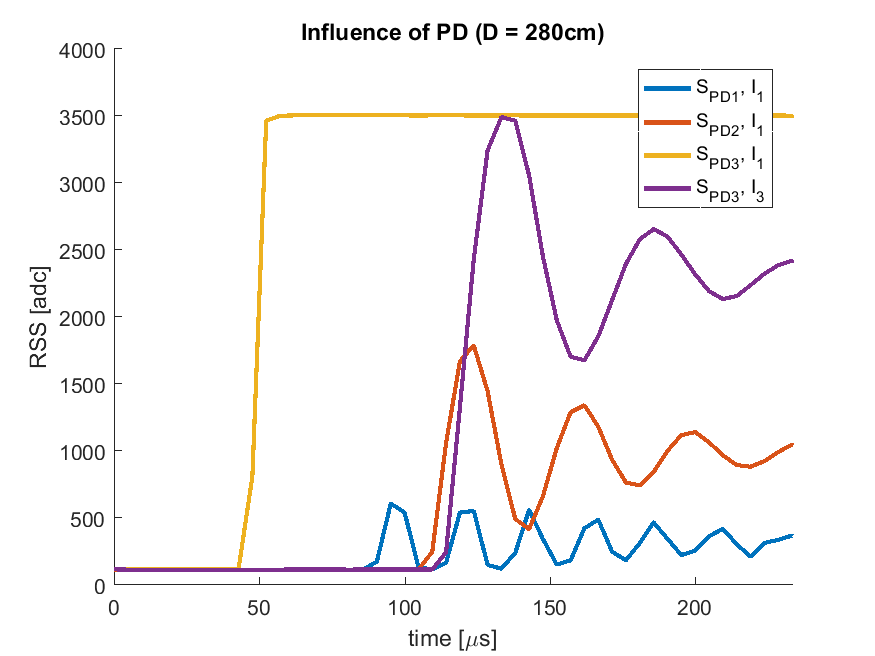
\includegraphics[width=60mm]{pics/InfluenceOfPD.png}}
	\caption{Several perceived flashes generated with different settings of $T_{on}$, $I_{LED}$, $D$ and $PD$.\label{fig:InfOf}}
\end{figure}

% properites checklist:
% - What happens if distance increases
%   + fig with multiple distances
% - What happens if t-on time increases
%   + fig with increasing t-on
% - What happens if intensity increases
%   + fig multiple 3 intensities
% sumarize in table 
% conclude:
% - 

\section{Flash features}
This section explores what kind of features can be extracted from a flash signal. It will then compare the methods based on required $T_{on}$, precision, the "Signal to Noise Ratio" (SNR) and computational complexity.

\subsection{Feature considerations}
The maximum of a flash response could contain useful information. Even though the light at the first maximum has not fully turned on yet, it still is some measure of the perceived light. This can be especially useful if the maximum of the flash always occurs at the exact same moment in time relative to the light turning on. If that's the case, then the maximum value of the first peak could provide us with enough information of the environment. If the maximum value of the first peak holds enough information, then a very small $T_{on}$ can be used to obtain this value, as decreasing $T_{on}$ does not significantly influence the height and form of the first peak.

Another possibility is the to remove the oscillation of the signal with a low pass filter and then take the maximum value of the filtered signal. This method less reliant on precise timing of the pulse. It also uses more samples of the signal and should therefore be able to obtain a value which better represents the reflections of the current environment than the maximum method. A downside to this method is that a filter designed to deal with one frequency of ripple, is not immediately suited to deal with the ripple frequencies of the other amplifiers

Another method considered is to use the surface underneath the flash. This method has the advantage of being both simple and flexible. It does not matter if $T_{on}$ is chosen big or small, it will always give a reliable result if $T_{on}$ is not changed. It also does not care about the ripple frequency of the amplifier. This method simply sums all information available to obtain a measure of the reflections.

The final possibility considered is the filtered sum method. It first uses a filter to smooth the signal to then calculate the surface underneath it. It also requires multiple filters to be designed (one for each $PD$ amplifier). It might however give a more detailed result than the filter method, as more information is used obtaining the data point.

\subsection{Feature comparison}
A test was created to compare the effectiveness of each feature with various settings in a full scale environment ($D = 280cm$). The test was executed as follows:
\begin{enumerate}[itemsep=-1ex]
	\item Set the parameters for the given test ($PD$, $I$, $T_on$).
	\item Move a highly reflective piece of cloth underneath the set-up at $185cm$ ($D = 95cm$).
	\item Move the piece of cloth underneath the setup again, but now from the other direction.
	\item Calculate the SNR of the received signal.
\end{enumerate}
If we refere to the 'SNR' in this thesis we mean the SNR as defined in equation \ref{eq:snr}. This equation calculates ratio between the standard deviation of the signal when noting is passing by and the absolute minimum and maximum of when something is. The higher the SNR, the easier it should be to distinguish between activity and no activity later on.

\begin{equation}
SNR(PD) = \left(\frac{\mu(PD_{NoEvent}) - min(PD_{event})}{\sigma(PD_{NoEvent})} + \frac{ max(PD_{event}) - \mu(PD_{NoEvent})}{\sigma(PD_{NoEvent})}\right)
\end{equation}
\begin{equation}
\label{eq:snr}
SNR(PD) = \frac{max(PD_{Event}) - min(PD_{Event})}{\sigma(PD_{NoEvent})} 
\end{equation}

The test was done with all combinations of $PD$ and $I$. Only the combinations of $PD_2, I_{1}$ and $PD3, I_{3}$ gave potential usable results at full scale as for other combinations the flash was invisible or too bright (saturation) to observe. Several consecutive captured features can be seen in the Figures \ref{fig:SimpleFeatures} and \ref{fig:complexFeatures}. These where then used to calculated the SNR for each scenario. An overview of all calculated SNR values can be seen in table \ref{SNR_results}.

Based on the results of the SNR test it was chosen to use the Filtered sum method with $T_{on} = 200\mu s$. This method gives better results than the maximum and filtered maximum methods because more measurements are used to determine the final value, leading to lower standard error. The reason that this method works better than the sum method lies in the fact that the filtered signal is better representation for the environment that the rippled signal. This can also be seen in the difference between the maximum and filtered maximum.

\begin{table}[]
	\centering
\begin{tabular}{l|lll|lll|}
	& \multicolumn{3}{c|}{SNR: $PD_2, I_1$} & \multicolumn{3}{c|}{SNR: $PD_3, I_3$} \\
	$T_{on}$         & $150 \mu s$ & $200\mu s$ & $250\mu s$ & $150\mu s$  & $20\mu s$  & $25\mu s$  \\ \hline
	Maximum          & 35          & 38         & 40         & 5           & 5          & 5          \\
	Filtered maximum & 39          & 65         & 66         & 20          & 27         & 33         \\
	Sum              & 45          & 75         & 95         & 18          & 20         & 26         \\
	Filtered sum     & 50          & 105        & 100        & 19          & 20         & 24        
\end{tabular}
	\caption{Overview of the test results.\label{SNR_results}}
\end{table}


\begin{figure}
	\centering     %%% not \center
	\subfigure[]{\label{fig:simple_PD2}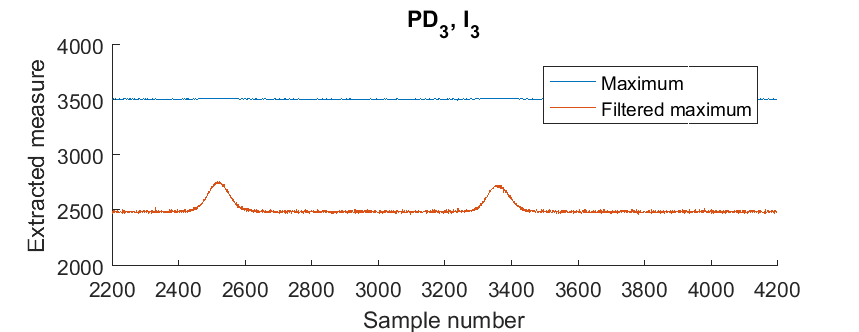
\includegraphics[width=60mm]{pics/SNR_simple_PD2.png}}
	\subfigure[]{\label{fig:simple_PD3}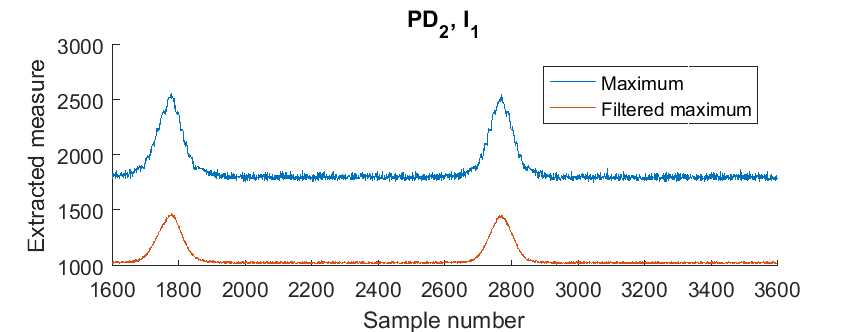
\includegraphics[width=60mm]{pics/SNR_simple_PD3.png}}
	\caption{Data extracted using the maximum and filtered maximum methods with $T_{on} = 250\mu s$.\label{fig:SimpleFeatures}}
\end{figure}

\begin{figure}
	\centering     %%% not \center
	\subfigure[]{\label{fig:complex_PD2}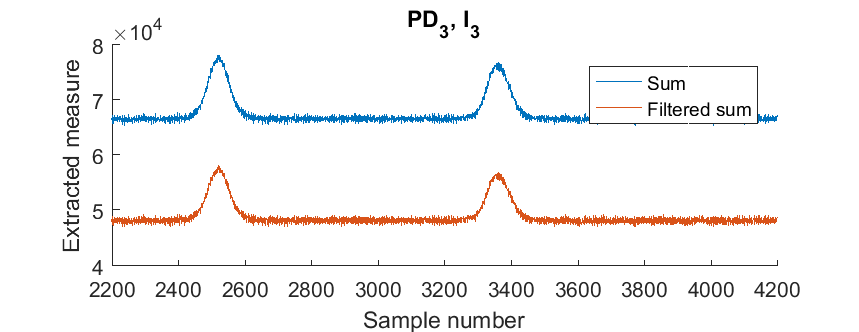
\includegraphics[width=60mm]{pics/SNR_complex_PD2.png}}
	\subfigure[]{\label{fig:complex_PD3}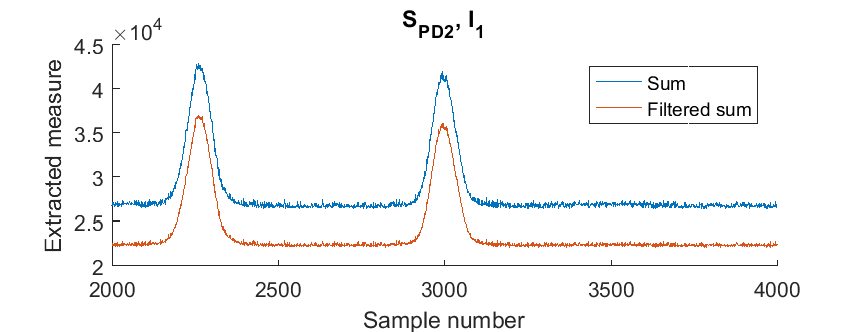
\includegraphics[width=60mm]{pics/SNR_complex_PD3.png}}
	\caption{Data extracted using the sum and filtered sum method with $T_{on} = 200\mu s$.\label{fig:complexFeatures}}
\end{figure}

\section{Flash period}
The final parameter to decide is the period of the signal, $T$. This value has no influence on the calculated SNR. It has however a clear influence on how much light is used by the system, as decreasing $T$ directly increases the amount of flashes which occur. We can't choose a too low value for $T$ as then users will observe flickering of the light. Another reason $T$ can't be chosen too low is that certain kind of noise still needs to be filtered out of the system. It is almost guaranteed that some 50Hz component will be seen in the signal, as long as its connected to the net. 

For these reasons, $T$ was chosen to be 800$\mu s$ restuling in a flash frequency of 125Hz. This value is more that the Nyquist frequency of the 50Hz and should therefore be filterable by the system. Even though literature recommends at least 200Hz to prevent the visibility of flickering, none was observed by 10 different test subjects with this setting of $T$.

\section{Conclusion}
The Flash analyser will run at a frequency of 125Hz, a $T_on$ of $200\mu s$ with maximum light intensity $I_1$ using the filtered sum method with $PD_2$ to extract information from the reflections. These settings provide the best found signal to noise ratio with the given platform. The next step for the project is creating an algorithm for the analyser, capable of analysing a set of consecutive flashes.
\chapter{Analyser}
\label{chp:Analyser}
This section will describe the path from the signal obtained in section \ref{sec:Method} to a proper detection algorithm, able to determine if something has changed in the environment or not. All algorithms will then be tested against a simulated signal.

\subsection{Simulation of the signal}
The first step in creating a proper algorithm, is to identify what signals are affecting the measurement, so a proper simulation set-up can be created. For this reason, equation \ref{eq:Pd_light} was devised. It shows the composition of the received signal \pmb{$PD$} after it's down sampled to 125Hz with the method described in section \ref{sec:Method}. The equation for $PD$ helps to understand what steps are required to create a reliable algorithm.

\begin{equation}
\label{eq:Pd_light}
PD = I_{L} \alpha + \sum_{i=1}^n I_{Edc_{n}} \beta_{n} + \sum_{i=1}^n I_{Eac{_n}} \gamma_{n} + N_{50Hz} + N(\mu,\sigma^2)
\end{equation}

The first part of the equation, "\pmb{$ I_{L} \alpha$}", is the amount of light generated by our luminaire ($I_{L}$), multiplied by some factor describing the environment from the point of view of the luminaire ($\alpha$). This signal typically occurs in two ways. The first is a person or object passing by. This can be approximated by the first or second half of a slow sinus period. The other way this signal can occur is if an object moves into range of the sensor, stops, and then stays still for a long time. This can be modelled as a sine wave, followed by constant, interrupting the wave. The wave is typically a low frequency signal between 0.25Hz and 2Hz (see section \ref{sec:Model}). An example of this signal can be seen in figure \ref{fig:SepparatedSignals}.

The second part of the equation, "\pmb{$\sum_{i=1}^n I_{Edc_{n}} \beta_{n}$}", describes the impact of all constant light sources ($I_{Edc_{n}}$), multiplied by the factor describing the environment from their point of view ($\beta$). An example of a constant light source is moonlight. The final factor involving light in the equation is \pmb{$\sum_{i=1}^n I_{Eac_{n}} \gamma_{n}$}. This describes all fluctuating light sources ($I_{Eac_{n}}$), multiplied once again by an environment describing factor from it's point of view ($\gamma_{n}$). This signal is typically 100Hz as most "old" lights blink or fluctuate at this frequency. Note that the sampling frequency is not twice as big as the sampled frequency, thus aliasing will occur at 25Hz ($= |F_{s} * 1 - F_{Analyze}| = 125 - 100 = 25Hz$)\cite{aliassing}. An example of these signals can be seen in figure \ref{fig:SepparatedSignals}.

The last two terms in the equation have nothing to do with light, but represent noise from all other sources. \pmb{$N_{50Hz}$} represents specifically 50Hz noise. This is powerline-noise picked up by the physical wire of connecting the photo-diode to the amplifier. Normally, line-noise is barely noticeable, but as all the signals are amplified by a 1000 times, it becomes a significant disturbance. The final part of the equation, \pmb{$N(\mu,\sigma^2)$}, is all the noise described in section \ref{subsec:noise}. An example of these signals can be seen in figure \ref{fig:SepparatedSignals}.

The only part of equation \ref{eq:PD} that holds information we can use is $I_{L} \alpha$, or more specifically, the changes of $\alpha$. For this reason, each of the methods described in this section focus on removing the other parts of the equation, or making changes of $\alpha$ more detectable.

\begin{figure}
	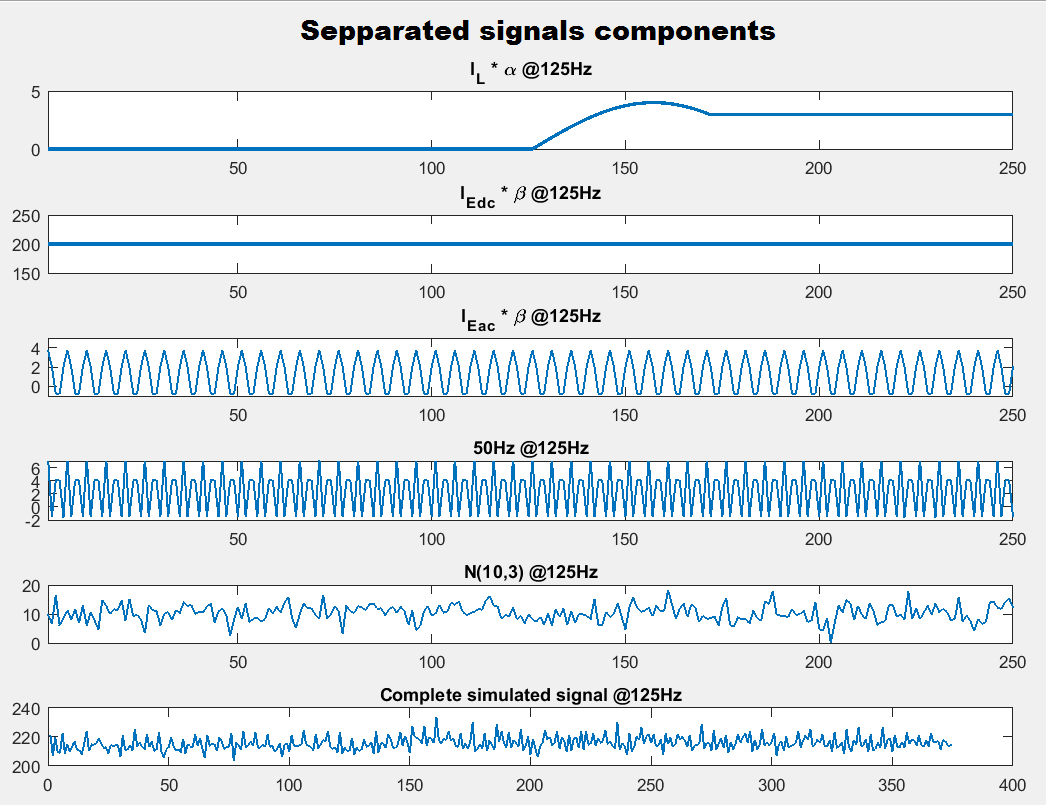
\includegraphics[width=\textwidth]{pics/sepparatedsignals.png}
	\caption{An example of what two seconds of all signal components look like when separated. The bottom signal shows all signals combined. Note that all signals where down sampled from the original sample rate of 200Khz (actual sample rate of the photo diode) to 125Hz(output speed of the sample unit).}
	\label{fig:SepparatedSignals}
\end{figure}

\subsection{Removing high frequency components}
\label{subsec:removeing_AC}
Filtering higher frequencies from a signal is a common challenge in signal processing. The signals we try to isolate ($I_{L}\alpha$, 0.25 to 2Hz) are far removed from the frequencies we are trying to suppress ($I_{Eac}$ at 100Hz and $N_{50Hz}$ at 50Hz). The most common method of doing this is by using digital filters. As only the lower frequencies are interesting, a low-pass filter seems to be ideal in this case. There is however one problem. $2 * I_{Eac}$ Is above our sampling frequency, and thus aliasing will occur. In this example it will appear as a 25Hz signal. This signal poses no real issue, as its still an order of magnitude away from the frequency of $ I_{L} \alpha$, and it can still be filtered with a steeper filter. This however, is not always the case in the real world. Any light manufacturer can create lights running at any frequency, and thus there is no guarantee that there won't be a light out there in the world, that can mess the algorithm up. In all other cases this filter probably works fine. Figure \ref{fig:FilterVSAllias} shows how a low-pass filter would remove the signals from the data.

\begin{figure}
	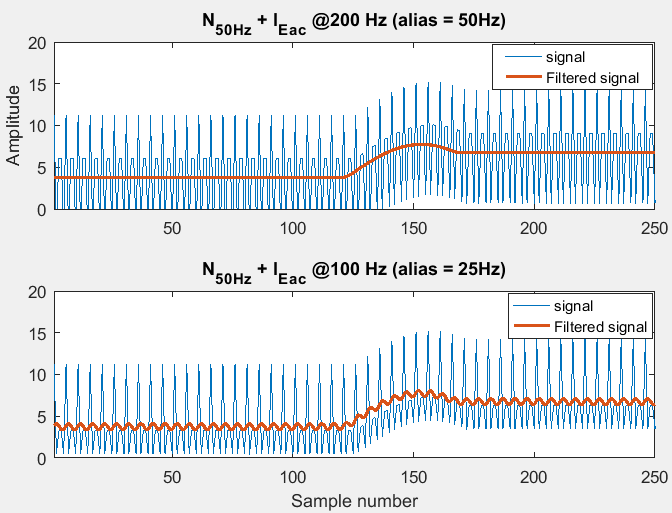
\includegraphics[width=\textwidth]{pics/FirFilter_vs_allias.png}
	\caption{A low-pass filter, filtering the $I_{Eac}$ and $N_{50Hz}$ signals.}
	\label{fig:FilterVSAllias}
\end{figure}

A completely other method of removing these high frequency components is the "$PD_{dark}$" method. This method uses the fact that the sensor set-up can do more than just sampling when the light ($I_{L}$) is turned on. It's also possible to take samples when the light is turned off. The components in such a sample are shown in equation \ref{eq:Pd_dark}. If this sample is obtained a short time away from the original $PD$ then the 50Hz and 100Hz values are roughly the same. Therefore subtracting $PD_{dark}$ from $PD$ gives the equation \ref{eq:Pd_light_dark}, resulting in a signal where $I_{Eac}$, $I_{Edc}$ and $N_{50Hz}$ have practically disappeared.
\begin{equation}
\label{eq:Pd_dark}
PD_{dark} = \sum_{i=1}^n I_{Edc_{n}} \beta_{n} + \sum_{i=1}^n I_{Eac{_n}} \gamma_{n} + N_{50Hz} + N(\mu,\sigma^2)
\end{equation}

\begin{equation}
\label{eq:Pd_light_dark}
PD - PD_{dark} = I_{L} \alpha + N(0,\sigma^2 + \sigma^2_{dark})
\end{equation}
The signals can't be filtered completely with this method though. This is because of the turn-off time of the LED (see section \ref{sec:Dimming and its consequences}), and the filters used to create a usable signal from the turning on and off of the LED (see section \ref{subsec:T-on_Time}). Both introduce a delay to the $PD_{dark}$ sample. Figure \ref{fig:Phaseshift} shows how much several signals get suppressed at various delay values.

Another downside of this method is that adding or subtracting two noisy signals, leads to signal with even more noise. In this case, an increase of approximately ($\sqrt{\sigma^2+\sigma^2} =$) $\sqrt{2} \sigma$\cite{@needref@}, as the $\sigma$ of $PD$ and $PD_{dark}$ are practically the same.

\begin{figure}
	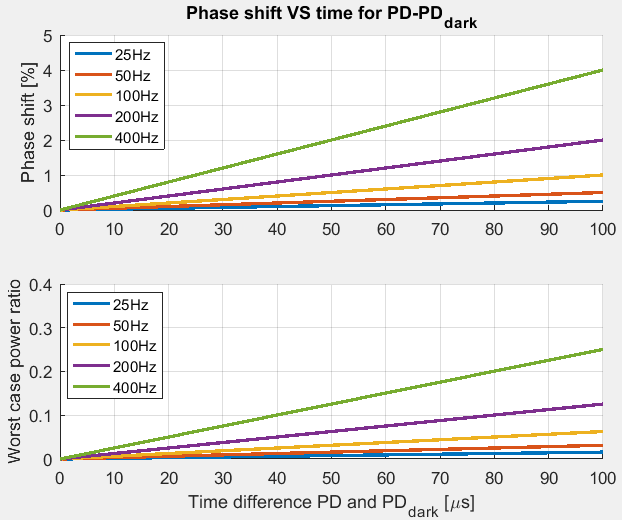
\includegraphics[width=\textwidth]{pics/PasheshiftVStime.png}
	\caption{The amount of phase shift that will occur.}
	\label{fig:Phaseshift}
\end{figure}

The huge selling point of this method in comparison to simply filtering, is that no aliasing of $I_{Eac}$ can occur. Another positive point, is that if a LED is specifically selected for it's a short turn off time, then this filter method is able to remove almost all disturbing sinusoid signals. 

\subsection{Detection threshold}
The first thing necessary to detect changes in $\alpha$ is a change detector, or with other words, if the signal has changed more than $X$, then we assume that the changes in the signal are not caused by noise, but by actual changes of $\alpha$ (the environment). from this point it is assumed that $I_{Eac}$ and $N_{50Hz}$ are no longer a significant part of the signal, as they can be practically removed by any of the methods described in section \ref{subsec:removeing_AC}.

A naive solution to this problem would be to sample a set amount of values when there are no objects in sight. Then, take the maximum and minimum of the sampled values and if the signal ever moves out of the range of the found values, activity is detected. Even though this might work consistently in a dark room (lab environment with no lights), it fails to work in a more realistic environment. If we for example introduce a slowly rising $I_{Edc}$ (e.g. moonlight), then the signal will eventually peak above the current maximum value and trigger a false detection.

Another way of tackling this problem would be to allow the minimum and maximum thresholds to move up and down with the mean of the signal. This results in two thresholds moving up and down together with the mean of the signal, and therefore ignores the slow changing $I_{Edc}$. The downside of this solution is that if the noise level ($N(\mu,\sigma^2)$) where to increases, then the signal would still cross the set threshold and trigger a false detection. The opposite is also true. If the noise level decreases, then the threshold would not scale back automatically and thus making it "deaf" to smaller changes in the signal.

This problem can be solved using the standard deviation of the signal as thresholds instead. A standard deviation scales up and down based on the deviation from the mean, meaning that if a lot of noise is present in the signal, then the detection borders would scale up and vice versa. The detection borders could be set on $\mu\pm T\sigma$, where $\mu$ is the mean, $\sigma$ is the standard deviation and $T$ is a factor determining width of the threshold

Using this method has another benefit. As the noise in our system ($N(\mu,\sigma^2)$) can be approximated with a normal curve (see section \ref{subsec:noise}), it allows us to control the amount of false positives perceived by the system by adjusting the $T$ parameter. How $T$ influences the chance of a false positive can be seen in table \ref{tab:Tresholds}.

\begin{table}
	\centering
	\label{tab:Tresholds}
	\begin{tabular}{cccl}
		\hline
		T   & Chance false positive & Single occurrence @125 Hz & Double occurrence @125Hz\\ \hline
		2   & 4.550026\%            & 0.18s                     & 0.69 days               \\
		3   & 0.269979\%            & 2.96s                     & 198.5 days              \\
		4   & 0.006334\%            & 126.3s                    & 1001 years              \\
		5   & 0.000057\%            & 1178.2s                   & 12199827 years          \\ \hline
	\end{tabular}
	\caption{Chance of a false positive occurring for several values of T, how often this would happen}
\end{table}



%Discuss fixed threshold
%note that this does not adjust to a slowly changing I_DC
%discuss variable threshold with mu and sigma
%show that this kind of works.
%show how scaling m influcences algorithem

\begin{figure}
	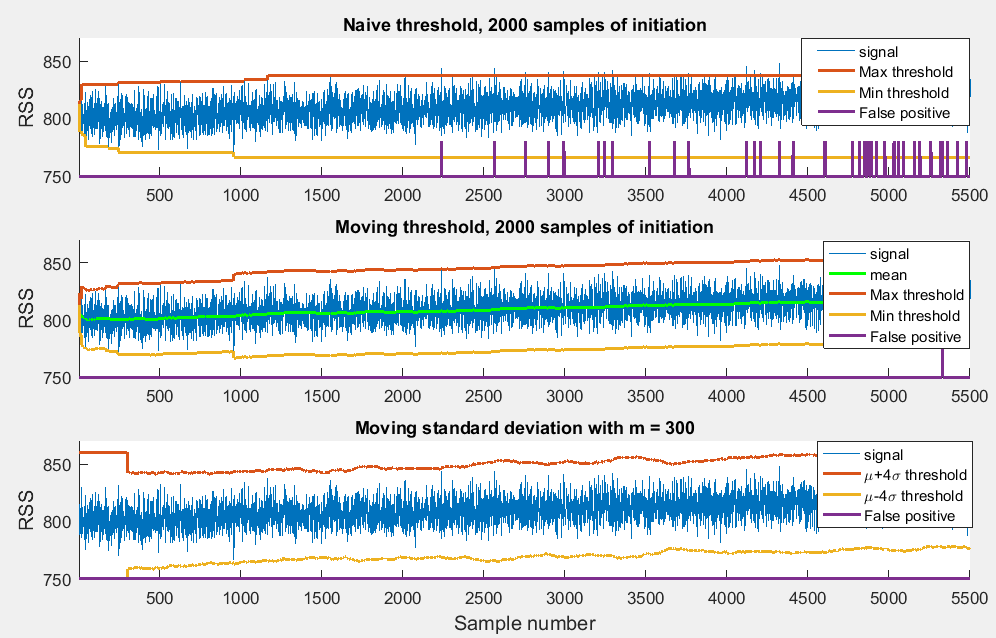
\includegraphics[width=\textwidth]{pics/NaiveVSsigmaThreshold.png}
	\caption{An example of how the discussed threshold algorithms respond to a slowly rising noisy signal.}
	\label{fig:Threshold}
\end{figure}

\subsection{Noise reduction}
The final thing that needs to be done, to make the algorithm more 

Averager \cite{Confidence_interval}

Scaling averager \cite{Confidence_interval}

\begin{figure}
	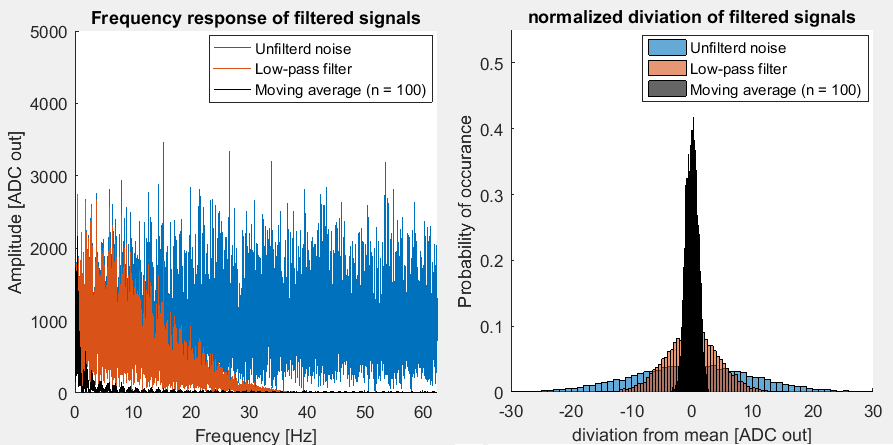
\includegraphics[width=\textwidth]{pics/FiltersVsNoise.png}
	\caption{Frequency response of the noise, the noise when filtered with a low-pass filter, and then noise when filtered with a moving average.}
	\label{fig:FilterVsNoise}
\end{figure}

\begin{equation}
\label{eq:SNR}
SNR = 1 = \frac{\mu * ss}{T * \frac{\sigma}{\sqrt{n}}} \Rightarrow n = \left(\frac{T * \sigma}{\mu*ss}\right)^2
\end{equation}

\begin{equation}
\label{SNR_2}
T * \frac{\sigma}{\sqrt{n}} = \mu * ss
\end{equation}




\subsection{Algorithm overview}
\begin{table}
	\centering
	\label{tab:Filters_summarized}
	\begin{tabular}{lllll}
		\hline
		Algorithm             &\vline $I_{Edc_{n}} \beta_{n}$ & $I_{Eac{_n}} \gamma_{n}$           & $N_{50Hz} $     & $N(\mu,\sigma^2)$    \\ \hline
		Low-pass filter       &\vline None                    & Removed (unless unfortunate alias) & Removed      & Reduced              \\
		$PD - PD_{dark}$      &\vline Removed                 & Removed                            & Removed         & $\sqrt2$ increase    \\
		Moving average        &\vline None                    & Reduced                            & Reduced         & Statistically reduced\\
		Scaling moving average&\vline None                    & Greatly reduced                    & Greatly reduced & Statistically reduced\\ \hline
	\end{tabular}
	\caption{Overview of all decent filter algorithms with their effects on each signal.}
\end{table}

\begin{figure}
	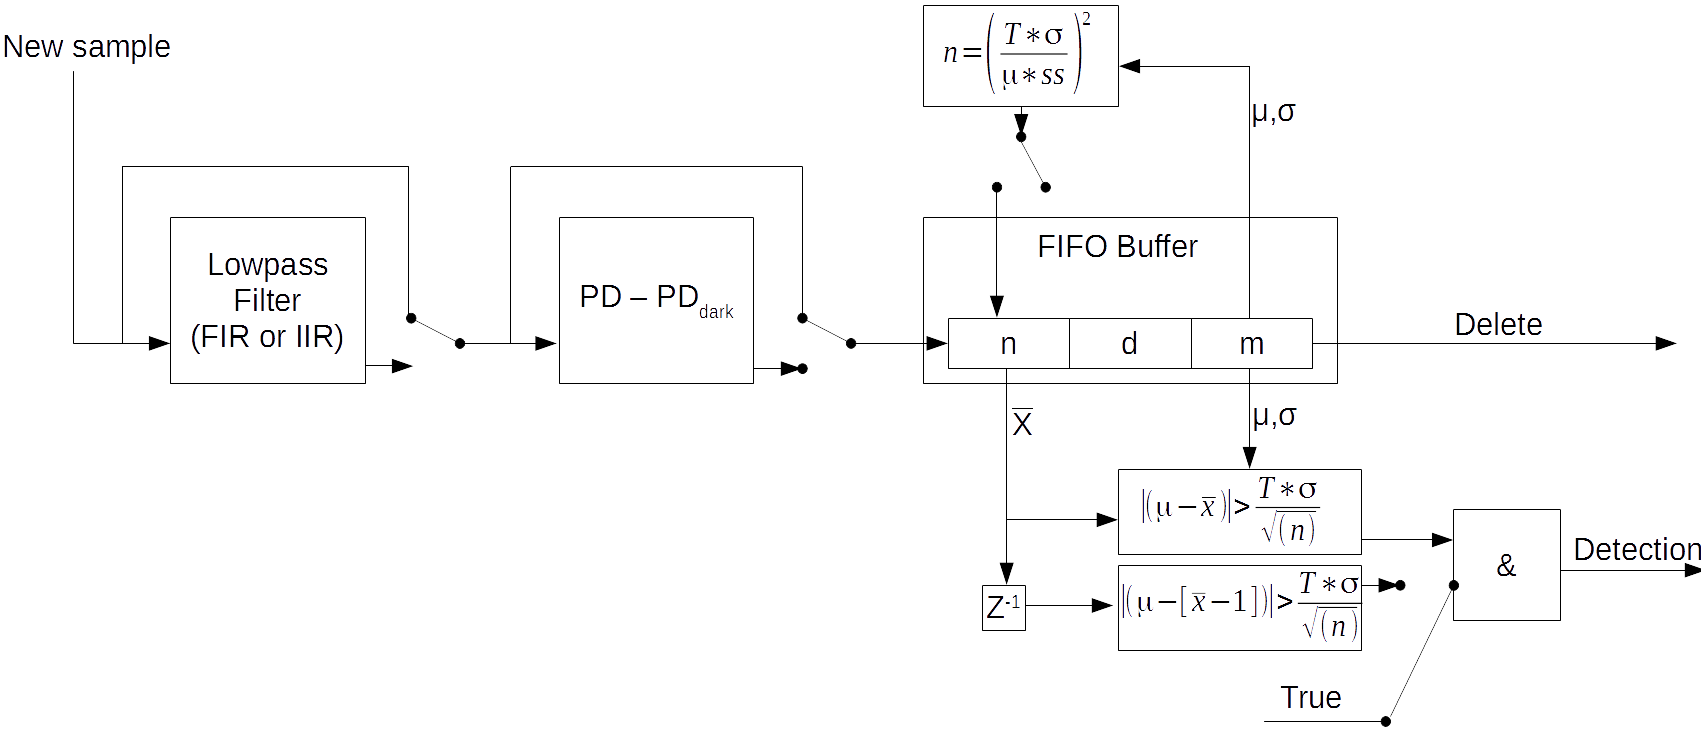
\includegraphics[angle=90,width=\textwidth]{pics/allSTDbasedAlgorithms_expanded.png}
	\caption{Overview of the algorithm.}
	\label{fig:fullAlgorithm}
\end{figure}

\chapter{System evaluation}
\label{System_evaluation}
%introduction - %current state
In the previous chapter an algorithm has been proposed, which should be capable of classifying a set of consecutive samples into two groups: Activity detected or no activity detected. The algorithm is however dependent on several parameters which have not been determined yet. The goal of this chapter is to find a set of parameters for the algorithm and evaluate the system using the algorithm tuned with those parameters.

This chapter starts with showing the test set-up which will be used to create a diverse dataset. This dataset will then be used to find parameters for the algorithm with which we evaluate the system. This chapter finishes with evaluating the performance of the system.

\section{Test set-up}
\label{dataset}
The test set-up used for evaluating and tuning the system can be seen in Figure \ref{fig:setup_a}. It shows the platform placed at 280cm above the ground in a room at night. Figure \ref{fig:signalsinestsetup} shows 15 seconds of received samples when the system was turned on. It can be seen that all described noise sources in section \ref{receivedsignals} where detected in the test environment.

Figure \ref{fig:setup_a} also shows three possible paths a pedestrian can walk. Path 1, the centre path, is placed directly under the light. Path 2 and 3 where placed at 30cm and 60cm from the centre path. The pedestrian was asked to wear one of the hoodies shown in Figure \ref{fig:setup_b} before traversing one of the paths. The different colours where used to ensure that the system was tested on various albedo's.

The ground where the pedestrian walked upon also varied. It was either a lacquered wooden floor or a blue carpet. The carpet on the floor produced a mostly diffuse reflection. The wooden floor produced a diffuse and spread reflection. These two floors were chosen to simulate how the system performs in different environments.

With the described set-up we created test-cases in the following manner:
\begin{enumerate}[itemsep=-1ex,topsep=0pt]
	\item Position a person at the beginning of a path.
	\item Start the gathering of samples and let the person wait for $\pm$ 35 seconds.
	\item After $\pm$ 35 seconds, the person starts walking
	\item When the person has reached the end of a path, stop the measurement.
\end{enumerate}
This procedure was repeated six times for each combination of floor material, path and hoodie colour, resulting in 180 unique test-cases. An example test-case can be seen in Figure \ref{TestScenario}. 

A test-case is split up in three sections. The first section (the first 25 seconds of data) serves to initialise the filters of the filter section and to fill the FIFO buffers used to calculate the moving $\sigma$ and moving $\mu$. After these 25 seconds the system can start detecting events. This is where section two starts. In this section, no events which should be detected by the algorithm are present. Then, after 10 to 15 seconds, section three begins when the person starts walking. In this section, the algorithm should trigger a detection.

\begin{figure}
	\centering     %%% not \center
	\subfigure[]{\label{fig:setup_a}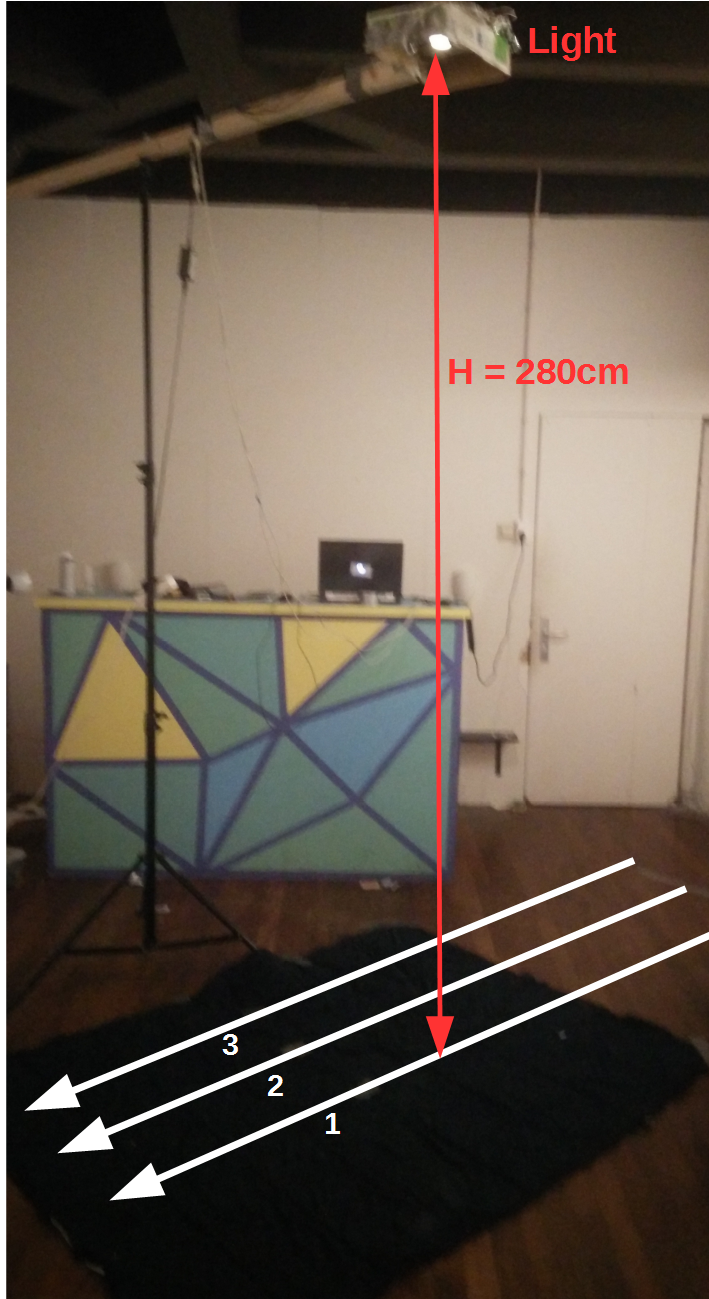
\includegraphics[width=50mm]{pics/Testsetup.png}}
	\subfigure[]{\label{fig:setup_b}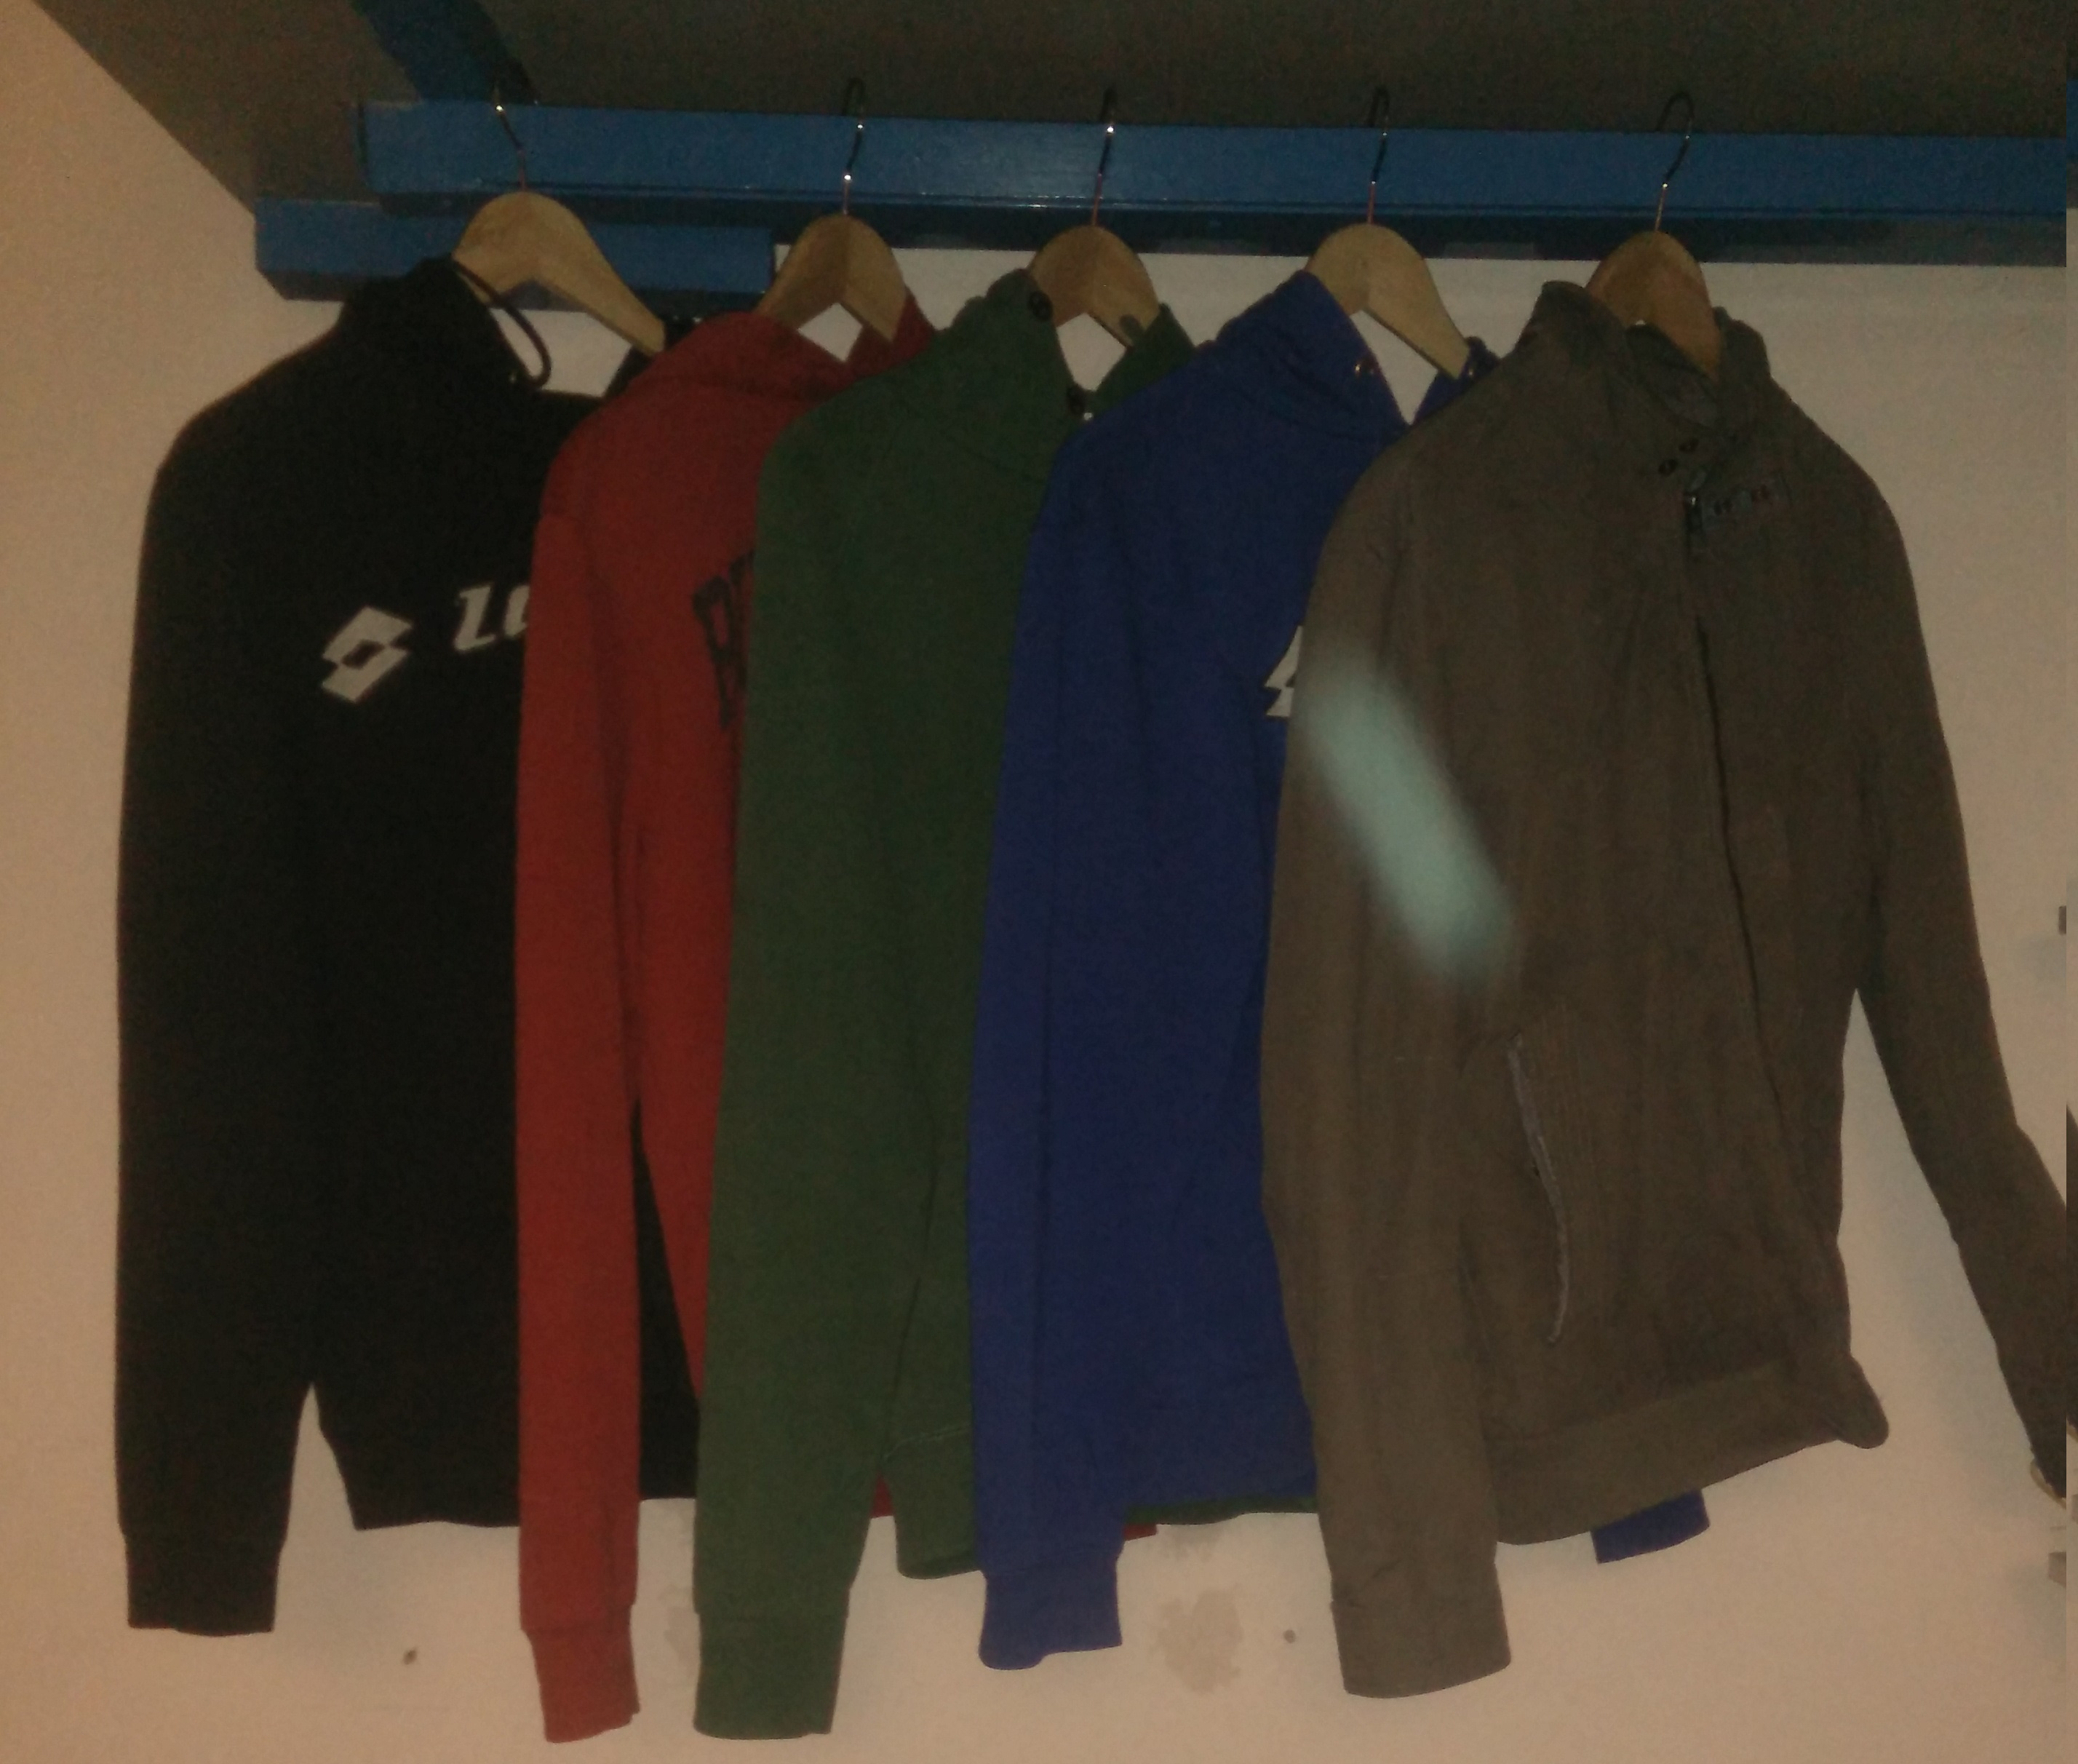
\includegraphics[width=70mm]{pics/Clothing.jpg}}
	\caption{(a) shows a picture of the test set-up with the blue carpet. The white arrows on the floor represent the three different paths the test subject walked over. The light is placed at a height of 2.8m. (b) shows the different clothing worn during the experiment (black, red, green, blue and grey).\label{fig:Testsetup}}
\end{figure}

\begin{figure}
	\centering     %%% not \center
	\subfigure[]{\label{fig:signals_Freq}\includegraphics[width=60mm]{pics/Signal_Final_chp.png}}
	\subfigure[]{\label{fig:signals_raw}\includegraphics[width=60mm]{pics/Freqplot_Final_chp.png}}
	\caption{(a) shows the received signal and (b) shows the frequency of this signal. $I_{Eac}$ and $N_{50Hz}$ are best seen in figure (b). $I_{Edc}$ is best observed in (a) (the slowly dropping signal).\label{fig:signalsinestsetup}}
\end{figure}

\begin{figure}
	\centering     %%% not \center
	\includegraphics[width=\textwidth]{pics/Examplescenario.png}
	\caption{An example scenario with the tree sections marked. The first section is used to initialise the filters, moving mean and moving standard deviation. The second section is use to check for false positives. The first section is used to check if the event gets detected properly. \label{TestScenario}}
\end{figure}

\section{Algorithm parameters}
A genetic algorithm (GA) was used to find parameters fo the algorithm. GA's are commonly used to generate high-quality solutions to optimization and search problems. In this case, we need to find good settings for the algorithm.

A GA needs two things to work. The first is a way to summarise a solution as a \textit{gene}. In our case, a gene is simply a set of numbers which represent the parameters of the algorithm. The range of allowed inputs can be seen in Table \ref{tbl:genes}.

\begin{table}[]
	\centering
	\begin{tabular}{l|cccccc}
		& d & m & l  & L  & T  & k  \\ \hline
		Min & 0 & 1 & 1  & 1  & 1  & -1 \\
		Max & 1000 & 1000 & 10 & 10 & 10 & 1 
	\end{tabular}
	\caption{Overview of the possible input genes for the genetic algorithm.\label{tbl:genes}}
\end{table}

The second thing a GA needs to work is a fitness function. This function evaluates the input gene and scores it based on its performance. In our case, we want a gene representing an algorithm, which detects persons passing by while not triggering when nobody passes by. This can be achieved by having the fitness function evaluate a dataset $S$ and counting the amount of test-cases where it correctly and incorrectly detects the pedestrians. The final fitness can be calculated with equation \ref{eq:ff}, where $TP$ is the amount of correct detections in the observed dataset, $FP$ is the amount of false detections in the observed dataset and $N$ represents the amount of test-cases in the dataset.

\begin{equation}
	Fitness = \frac{TP - FP}{N} \cdot 100\%
	\label{eq:ff}
\end{equation}

The described fitness function was used to train two separate algorithms. The first algorithm $ALG_1$ was found using dataset $S_1$, which contained the 90 test-cases created with the wooden floor. The second algorithm trained, $ALG_2$, was found using dataset $S_2$, which contained the 90 test-cases created with the carpet. The found algorithms can be seen in Table \ref{Found_settings}.

\begin{table}[]
	\centering
\begin{tabular}{l|llllll|l}
	              & d   & m   & l & L  & T   & k    & Fitness \\ \cline{1-8} 
	$ALG_1$       & 980 & 890 & 7 & 9  & 4.5 & 0.2  & 91\%    \\
	$ALG_2$       & 860 & 980 & 8 & 10 & 5.9 & -0.7 & 83\%
\end{tabular}
	\caption{The settings found with the genetic algorithm. $STD_1$ was trained with dataset $S_1$ and $STD_2$ was trained with dataset $S_2$.\label{Found_settings}}
\end{table}

\section{Evaluation}
The two found algorithms where evaluated against three different datasets: $S_1$, $S_2$ and $S_3$. $S_3$, is the union of $S_1$ and $S_2$, and contains all 180 test-cases. Results of this evaluation can be seen in Table \ref{tbl:Scoringresults}. We are aware that evaluating the algorithm with the dataset it was trained with gives biased results, but they were added for the sake of completeness. The most interesting sections of the table are marked blue. These sections show the results of testing $ALG_1$ on $S_2$ and $ALG_2$ on $S_1$. It can be seen that both algorithms seem to perform reasonably well as they achieve a fitness of over 75\%.

\begin{table}[]
	\hskip-2.7cm
\begin{tabular}{l|lll|lll|lll}
	& \multicolumn{3}{c|}{$S_1$}                                                                         & \multicolumn{3}{c|}{$S_2$}                                                                           & \multicolumn{3}{c}{$S_1 \cup S_2$} \\ \hline
	Algorithm & TP (\%)                           & FP (\%)                         & Fitness                      & TP (\%)                           & FP (\%)                           & Fitness                      & TP (\%)      & FP (\%)   & Fitness  \\ \hline
	$ALG_1$   & 86 (96\%)                         & 4 (4\%)                         & 91\%                         & \cellcolor[HTML]{BBDAFF}81 (90\%) & \cellcolor[HTML]{BBDAFF}11 (12\%) & \cellcolor[HTML]{BBDAFF}78\% & 167 (93\%)   & 15 (8\%)  & 84\%     \\
	$ALG_2$   & \cellcolor[HTML]{BBDAFF}84 (93\%) & \cellcolor[HTML]{BBDAFF}3 (3\%) & \cellcolor[HTML]{BBDAFF}90\% & 81 (90\%)                         & 6 (7\%)                           & 83\%                         & 165 (91\%)   & 9 (5\%)   & 87\%    
\end{tabular}
	\caption{Results of testing the found algorithms against all datasets.\label{tbl:Scoringresults}}
\end{table}

This method however, does not give a good representation of how the system performs in the real world, as the fitness score of an algorithm does not tell us how much energy is saved and how much of the bypassing persons are actually detected. A better way to gain insight in the performance of this system is with recall and the false positive ratio.

Recall, $R$, is defined in equation \ref{eq:precsion/recall} and gives us insight in how often the system fails to detect an object passing by. $R = 1$ means that all events are detected were $R = 0$ means that none of the pedestrians are detected. The false positive ratio, $FP_r$, is defined in equation \ref{eq:precsion/recall} and gives us insight in how often the system makes a false detection. Because it's known how much time we observe when we determine if a false positive occurs, we can calculate the chance on a false positive per minute with equation \ref{eq:FPratio}.

If we evaluate the algorithms with these metrics, we see that $ALG_1$ has a 18\% chance on a false positive every minute and $ALG_2$ a 54\% chance. These numbers show that the system, with the current algorithm settings, makes too much mistakes and won't be usable to save energy. It is however possible to manually adjust the found parameters to better suit our system.

\begin{equation}
\label{eq:precsion/recall}
Recall = R = \frac{TP}{TP + FN}
\quad
FP_{r} = \frac{FP}{FP+TN}
\end{equation}

\begin{equation}
\label{eq:FPratio}
P_{FP/minute} = 1 - \left(1 - \frac{FP}{FP+TN}\right)^{6t}
\end{equation}

\begin{figure}
	\centering     %%% not \center
	\subfigure[]{\label{fig:STDs1_s2}\includegraphics[width=60mm]{pics/STDs1_s2.png}}
	\subfigure[]{\label{fig:STDs2_s1}\includegraphics[width=60mm]{pics/STDs2_s1.png}}
	\caption{The false positive ratio and recall plotted as a function of $T$, for both created algorithms. \label{STDx_vs_Sx}}
\end{figure}

The easiest way to manually adjust the algorithm is by changing the value of $T$. $T$ directly influences the detection threshold. Raising $T$ will by definition, decrease the amount of false positives (lowering $FP_r$) and true positives (lowering recall) we detect. Two plots, showing $R$ and $FP_r$ as a function of $T$ for both algorithms can be seen in Figure \ref{STDx_vs_Sx}. 

In these plots it can be seen $FP_r$ drops fairly fast if $T$ increases, until $FP_r$ reaches $0.1$. From this point, $T$ needs to increase a lot, to further increase $FP_r$ significantly. This is because the false positives in these test-cases are not caused by the previously described noise sources but by artefacts occurring in the test data. One of such artefacts is shown in Figure \ref{fig:resforfailure} at $t = 32s$.

These artefacts are caused by slight fluctuations in the power supply of the flash receiver. This part of the system is powered by an USB port of the analyser. Slight voltage drops in the USB ports are common but usually no problem as the changes are minimal. If they get amplified 5600 times however, they become visible and will influence the measurements of the photodiode. this problem could be solved by powering the system with a battery or a very stable power supply. This is however no longer possible for this project due to time constraints.

It is however still possible to ignore the artefacts by choosing an ideal value for $T$ with the help of Figure \ref{STDx_vs_Sx}. For example, if we want a system which does not trigger any false positives (e.g. $FP_r = 0$), then we have to choose $T = 12$ for $ALG_1$ and $T = 9.6$ for $ALG_2$. This leads to the detection results shown in Table \ref{tbl:P=1}. It can be seen that the detection ratio of persons walking directly under the light is good (90\% and 100\%), but the further we move away from the centre, the worse the detection ratio (recall) becomes.

\begin{table}[]
	\centering	
\begin{tabular}{l|ccc|ccc}
	& \multicolumn{3}{c|}{$ALG_{carpet} \rightarrow FP_r = 0$} & \multicolumn{3}{c}{$ALG_{wood} \rightarrow FP_r = 0$} \\
	& R Lane 1        & R Lane 2        & R Lane 3        & R Lane 1         & R Lane 2        & R Lane 3        \\ \hline
	Red    & 1               & 1               & 1               & 1                & 0.5             & 0.83            \\
	Black  & 1               & 0.33            & 0               & 1                & 0.5             & 0               \\
	Green  & 1               & 0.83            & 0.67            & 1                & 0.83            & 0.83            \\
	Blue   & 1               & 0.83            & 0               & 1                & 0.83            & 0.17            \\
	Grey   & 0.5             & 1               & 0.5             & 1                & 1               & 1               \\ \hline
	Total: & 0.9             & 0.8             & 0.43            & 1                & 0.73            & 0.57           
\end{tabular}
	\caption{Overview of the performance of $ALG_2$ when tested on $S_1$ and $ALG_1$ on $S_2$ with $T$ set so that $FP_r = 0$. \label{tbl:P=1}}
\end{table}

The amount of detections can be increased by lowering $T$, but this leads to more false classifications by the system. For example, if we allow a false positive ratio of 0.05 (26\% chance on a false positive every minute), we can greatly increase the amount of true detections. This can be seen in Table \ref{tbl:P=0.95}. If we look at the results by colour in this table, we can see that the system has trouble detecting pedestrians wearing blue and black clothing. This makes sense. The black clothing does not reflect a lot of light compared to the other colours and is therefore less visible to the system. The low detection ratio of blue clothing can be explained with the help of Figure \ref{fig:Colours}. This Figure shows the colour spectrum of the used LED. It can be seen that considerably less blue light is generated by the LED than the other tested colours. It therefore makes sense that the signals created with the blue hoodie are less visible to the system.

\begin{table}[]
	\centering
	\begin{tabular}{l|ccc|ccc}
	& \multicolumn{3}{c|}{$ALG_2(S_1) \rightarrow FP_r = 0.05$} & \multicolumn{3}{c}{$ALG_1(S_2) \rightarrow FP_r = 0.05$} \\
		& R Lane 1             & R Lane 2             & R Lane 3             & R Lane 1           & R Lane 2           & R Lane 3          \\ \hline
		Red    & 1                    & 1                    & 1                    & 1                  & 0.5                & 0.83              \\
		Black  & 1                    & 0.83                 & 0.67                 & 1                  & 0.83               & 0.17              \\
		Green  & 1                    & 1                    & 1                    & 1                  & 0.83               & 1                 \\
		Blue   & 1                    & 1                    & 1                    & 1                  & 0.83               & 0.5               \\
		Grey   & 1                    & 1                    & 1                    & 1                  & 1                  & 1                 \\ \hline
		Total: & 1                    & 0.97                 & 0.93                 & 1                  & 0.8                & 0.7              
	\end{tabular}
	\caption{Overview of performance of $ALG_2$ on $S_1$ and $ALG_1$ on $S_2$ with $T$ set so that $FP_r = 0.05$.\label{tbl:P=0.95}}
\end{table}

\begin{figure}
	\centering     %%% not \center
	\subfigure[]{\label{fig:resforfailure}\includegraphics[width=60mm]{pics/ReasonForFailure.png}}
	\subfigure[]{\label{fig:Colours}\includegraphics[width=60mm]{pics/Colourspectrum.png}}
	\caption{(a) shows an example of an artefact at $t = 32s$, caused by fluctuations in the power supply. (b) shows the frequency spectrum of the light emitted of the LED used by the system.\label{fig:explanations}}
\end{figure}

\section{Conclusion}
We have developed a method which is capable of analysing a set of consecutive flashes with the goal of detecting bypassing pedestrians, even when a considerable amount of noise sources are mixed in the signal. The created filters and algorithms managed to achieve a combined recall between 0.73 and 0.9 depending on the setting of $T$ and the amount of allowed false positives ratio (0 to 0.05). The system has shown to work on two floors types and on several colours of clothing.

We are aware that the evaluation of the system is minimal, as the system was with a limited dataset. The algorithm was then tweaked by adjusting $T$, to fit the data even more. This method of evaluation at least shows the potential of the system. It also manges to expose some key flaws. It has trouble detecting pedestrians wearing black and blue clothing and has regular false detections if we try to achieve a high detection ratio because of a flaw in the hardware design.

The most direct approach to deal with the identified problems is to improve the hardware design. Changing the LED with one, which emits light more evenly distributed along all wavelengths, will improve the detection ratio of bypassers wearing blue. Changing the power supply and implementing the full system with a detected processor will remove the artefacts and decrease the complexity of the project. It will also allow for the wires to the photodiodes to be shortened and therefore reducing the total amount of noise received by the system.

% CONCLUSIONS AND FUTURE WORK
\chapter{Conclusions and Future Work}
\label{chp:conclusionsandfuturework}

\section{Conclusions}
% introduction
This thesis proposed a new method for activity detection while only using visible light and a photodiode with the goal of saving energy. This can be achieved by measuring reflections of light with a photodiode, produced by a light. A model has shown that the changes in reflection are measurable by a photodiode if a person walks by.

A flash does not appear as a perfect square to a photodiode. Therefore, a method was created to extract the most relevant features from a flash. These features where then analysed by a newly created algorithm capable of analysing consecutive flashes.

A prototype has been made with off-the-shelve parts, implementing the proposed system. The prototype was created to work in a hallway of an university. It showed to detect 100\% of all persons directly walking underneath the light, no matter the colour of their clothing or environment the system was placed in. 86.5\% and 76.5\% of pedestrians where detected at 30 and 60 cm from the centre of the set-up. The system has a 25\% chance on a false detection every minute, which is caused by poor build quality of the prototype.

Even though the prototype has a relatively high false positive ratio, it serves as a good proof of concept for detecting activity with short flashes of visible light.

\section{Future Work}
The presented work serves as a proof of concept for detecting activity in the line of sight of an LED. I personally think that the potential of this system is huge, especially if a dedicated platform is created, as most shortcomings of the current prototype can be solved if a better platform is built. Below I have listed several ideas for future research.

\begin{itemize}
	\item \textbf{Multiple units in one room} - The algorithm is currently designed for a stand-alone device. If we would hang multiple of these systems in the same room then it's likely that some of the light flashes overlap and trigger a false positives regularly. This problem could be solved by having each detector flash in another timeslot, but this requires more research.
	\item \textbf{Tracking} - The system is currently only detecting activity. It could also be expanded for other purposes. It might for example be possible to use multiple photo diodes, lenses or field of view blockers to track bypassing pedestrians.
	\item \textbf{A dark sensing network} - Multiple working units in one room is nice, but multiple units working together to track, predict and illuminate the path of a pedestrian is nicer. This could be achieved by having the devices communicate using the flashes already generated by the device (visible light communication).
\end{itemize}

% BIBLIOGRAPHY
%#define SORTED 1
\bibliographystyle{bib/latex8}
\bibliography{bib/mycollection}

\appendix

\chapter{Code repository}
\label{app_repository}
This appendix is the github repository where all the raw data, code and MATLAB scripts can be found, used to create this thesis. It can be found at:  \url{https://github.com/hkleingeld/DarkSensing}.


\chapter{Raw Model results}
\label{app:RawModelResults}
This appendix contains the raw results of the model.

\begin{table}[]
	\hspace{-15mm}
	\label{tab:results_hallway}
	\begin{tabular}{llllllllll}
		y   & H                         & \begin{tabular}[c]{@{}l@{}}min\\ $\alpha = 0.2$\end{tabular} & \begin{tabular}[c]{@{}l@{}}max\\ $\alpha = 0.2$\end{tabular} & \begin{tabular}[c]{@{}l@{}}min\\ $\alpha = 0.3$\end{tabular} & \begin{tabular}[c]{@{}l@{}}max\\ $\alpha = 0.3$\end{tabular} & \begin{tabular}[c]{@{}l@{}}min\\ $\alpha = 0.4$\end{tabular} & \begin{tabular}[c]{@{}l@{}}max\\ $\alpha = 0.4$\end{tabular} & \begin{tabular}[c]{@{}l@{}}min\\ $\alpha = 0.5$\end{tabular} & \begin{tabular}[c]{@{}l@{}}max\\ $\alpha = 0.5$\end{tabular} \\ \cline{3-10} 
		0m   & \multicolumn{1}{l|}{1.4m} & -0.08 & 0.70  & -0.03 & 1.30  & 0     & 1.90  & 0     & 2.50  \\
		& \multicolumn{1}{l|}{1.6m} & -0.07 & 1.60  & -0.02 & 2.66  & 0     & 3.73  & 0     & 4.80  \\
		& \multicolumn{1}{l|}{1.8m} & -0.06 & 3.46  & -0.01 & 5.54  & 0     & 7.61  & 0     & 9.69  \\
		0.2m & \multicolumn{1}{l|}{1.4m} & -0.05 & 0.65  & -0.01 & 1.17  & 0     & 1.70  & 0     & 2.23  \\
		& \multicolumn{1}{l|}{1.6m} & -0.05 & 1.34  & 0     & 2.22  & 0     & 3.11  & 0     & 3.99  \\
		& \multicolumn{1}{l|}{1.8m} & -0.04 & 2.64  & 0     & 4.24  & 0     & 5.83  & 0     & 7.43  \\
		0.4m & \multicolumn{1}{l|}{1.4m} & -0.07 & 0.28  & -0.02 & 0.59  & 0     & 0.90  & 0     & 1.21  \\
		& \multicolumn{1}{l|}{1.6m} & -0.07 & 0.56  & -0.02 & 1.01  & 0     & 1.46  & 0     & 1.91  \\
		& \multicolumn{1}{l|}{1.8m} & -0.07 & 0.91  & -0.02 & 1.59  & 0     & 2.26  & 0     & 2.93  \\
		0.6m & \multicolumn{1}{l|}{1.4m} & -0.08 & 0.04  & -0.03 & 0.18  & -0.01 & 0.33  & 0     & 0.47  \\
		& \multicolumn{1}{l|}{1.6m} & -0.09 & 0.09  & -0.04 & 0.27  & -0.01 & 0.44  & 0     & 0.62  \\
		& \multicolumn{1}{l|}{1.8m} & -0.10 & 0.05  & -0.05 & 0.26  & -0.01 & 0.47  & 0     & 0.68 
	\end{tabular}
	\caption{Differences with baseline (no object) for each simulated situation}
\end{table}

\begin{table}[]
	\centering
	\label{tab:results_street_car}
	\begin{tabular}{llllll}
		y & Colour & \begin{tabular}[c]{@{}l@{}}min\\ $\alpha = 0.06$\end{tabular} & \begin{tabular}[c]{@{}l@{}}max\\ $\alpha = 0.06$\end{tabular} & \begin{tabular}[c]{@{}l@{}}min\\ $\alpha = 0.14$\end{tabular} & \begin{tabular}[c]{@{}l@{}}max\\ $\alpha = 0.14$\end{tabular} \\ \cline{3-6} 
			1.5m & \multicolumn{1}{l|}{Silver} &  &  &  &  \\
			& \multicolumn{1}{l|}{Black} &  &  &  &  \\
			& \multicolumn{1}{l|}{Red} &  &  &  &  \\
			4.5m & \multicolumn{1}{l|}{Silver} &  &  &  &  \\
			& \multicolumn{1}{l|}{Black} &  &  &  &  \\
			& \multicolumn{1}{l|}{Red} &  &  &  & 
	\end{tabular}
	\caption{Differences with baseline (no object) for each simulated situation}
\end{table}

\begin{table}[]
	\centering
	\label{tab:results_street_human}
	\begin{tabular}{llllll}
		\begin{tabular}[c]{@{}l@{}}Object\\ albedo\end{tabular} & H & \begin{tabular}[c]{@{}l@{}}min\\ $\alpha = 0.06$\end{tabular} & \begin{tabular}[c]{@{}l@{}}max\\ $\alpha = 0.06$\end{tabular} & \begin{tabular}[c]{@{}l@{}}min\\ $\alpha = 0.14$\end{tabular} & \begin{tabular}[c]{@{}l@{}}max\\ $\alpha = 0.14$\end{tabular} \\ \cline{3-6} 
		0.1 & \multicolumn{1}{l|}{1.8m} &  &  &  &  \\
		& \multicolumn{1}{l|}{1.6m} &  &  &  &  \\
		& \multicolumn{1}{l|}{1.4m} &  &  &  &  \\
		0.4 & \multicolumn{1}{l|}{1.8m} &  &  &  &  \\
		& \multicolumn{1}{l|}{1.6m} &  &  &  &  \\
		& \multicolumn{1}{l|}{1.4m} &  &  &  & 
	\end{tabular}
	\caption{Differences with baseline (no object) for each simulated situation}
\end{table}
\chapter{Flash analyser schematics}
\label{app_schematics}
This appendix contains pictures of electronic schematic created for specifically the flash analyser. Schematics of the processor boards where not added, as only small changes small modifications (see section \ref{chp:Platform}) where made to these boards. The original scematics can be found at:
\begin{itemize}
    \item Flash analyser - \url{https://github.com/LennartKlaver/SDVN1} 
    \item LED controller - \url{https://www.arduino.cc/en/uploads/Main/arduino-uno-schematic.pdf}
\end{itemize}


\section{LED driver}
\begin{figure}[!h]
	\includegraphics[width=\textwidth]{pics/LED_Driver.png}
	\caption{Drivers used to drive the LED.}
	\label{fig:LED_Driver}
\end{figure}

\section{Interfaces between components}
@TODO!

\end{document}

